\documentclass[a4paper,12pt]{article}                                         % Schriftgröße, Layout, Papierformat, Art des Dokumentes
\usepackage[left=3cm,right=2cm,top=2cm,bottom=2cm,includehead]{geometry}      % Einstellungen der Seitenränder
%\usepackage{ngerman}                                                          % neue Rechtschreibung
\usepackage[ngerman]{babel}                                             % deutsche Silbentrennung                                                % Umlaute
\usepackage[hyperfootnotes=false, pdfborder={0 0 0}]{hyperref}                                   % pfd-Output [Fußnoten nicht verlinken]
\usepackage[nottoc]{tocbibind}                                                % Inhaltsverzeichniserweiterung (Inhaltsverzeichnis selbst ausblenden)
\usepackage{makeidx}                                                          % Index
%\usepackage[intoc]{nomencl}                                                   % Abkürzungsverzeichnis
\usepackage{fancyhdr}           	                                          % Fancy Header
\usepackage{pdfpages}															% 
\usepackage{amsmath}                                                          % Zurücksetzen der Tabellen- und Abbildungsnummerierung je Sektion
\usepackage[labelfont=bf,aboveskip=1mm]{caption}                              % Bild- und Tabellenunterschrift (fett)
\usepackage{setspace}                                                         % Zeilenabstand (vor footmisc laden!)
\usepackage[bottom,multiple,hang,marginal]{footmisc}                          % Fußnoten [Ausrichtung unten, Trennung durch Seperator bei mehreren Fußnoten]
\usepackage{wrapfig}
\usepackage{nomencl} % Für das Symbolverzeichnis
\usepackage{chngcntr} % Für die Nummerierung der Formeln in separaten Dateien
\usepackage{import} % Zum Einbinden von externen Dateien
% Umfließende Grafiken und Tabellen
\usepackage{graphicx}                                                         % Grafiken
\usepackage{tabularx}                                                         % erweiterte Tabellen
\usepackage{longtable}                                                        % mehrseitige Tabellen
\usepackage{color}                                                            % Farben
\usepackage{enumitem}                                                         % Befehl setlist (Zeilenabstand für itemize Umgebung auf 1 setzen)
\usepackage{listings}                                                         % Quelltexte
\usepackage{zref}                                                             % Verweise (Anhangsverweise)
\usepackage{wasysym}
\usepackage{amssymb}
\usepackage{float}
\usepackage{xspace}
\widowpenalty=300
\clubpenalty=300
\usepackage{multicol}
\usepackage{booktabs}
\usepackage{siunitx}
\RequirePackage{multirow}
\RequirePackage{longtable}
\RequirePackage{mwe}
\RequirePackage{listings}    
\RequirePackage{etoolbox} 


\usepackage{float}
\usepackage{adjustbox}
\usepackage{multirow}
\usepackage{comment}
\usepackage{longtable}
\usepackage{caption}
\usepackage{subcaption}
\usepackage{graphicx}
\usepackage{hanging}
\usepackage[printonlyused,withpage]{acronym}

%%%%%%%%%%%%%%%%%%%%%%%%%%%%%%%%%%%%%%%%%%%%%%%%%%%%%%%
%% Konfiguration %%
\def\myType{0}
%% 0=Projektarbeit   %%
%% 1=Bachelorarbeit  %%
%% 2=sonstige Arbeiten   %%
%% 3=sonstige Arbeiten mehrere Autoren  %%

\def\myTopic{}
\def\mySubTopic{Optimierung und Implementierung eines Artikel-Empfehlungssystems für die SV-Gruppe auf der Google Cloud Platform}

\def\myStudyProgram{Data Science und künstliche Intelligenz}         % Studiengang
\def\myNeedForFieldOfStudy{0} % Gibt an ob eine Studienrichtung benötigt wird
%% 0=keine Studienrichtung %%
%% 1=Studienrichtung %%
\def\myFieldOfStudy{Data Science und künstliche Intelligenz}         % Studiengangsrichtung

\def\myAutor{Finn Hertsch}
\def\myCourse{RV-WDS124}
\def\myProf{Dr. Andreas Heusler}
\def\myCompany{Schwäbischer Verlag GmbH \& Co. KG Drexler, Gessler}
\def\myCompanion{Mario Pfob}            % Begleitperson des dualen Partners
\def\myEndDate{30.09.2025}              % Abgabefrist


%% Projektarbeit %%
\def\myProjNumber{1}          % [1|2]

%% Bachelorarbeit %%
\def\myTypeOfBachelor{}       % [Arts|Science]

%% sonstige Arbeiten %%
\def\myTypeOfWork{}           % [Seminararbeit|Projektdokumeantation|...]
\def\myModule{}               % Modulname
\def\myNames{0}               % Gibt an ob mehrere Personen an der Arbeit mitwirken
%% 0=Einzahl %%
%% 1=Mehrzahl %%

%% Konfiguration der Verzeichnisse %%
% für alle folgenden Konfigurationen gilt: 0=kein Verzeichnis | 1=Verzeichnis %

\def\myAbrevationDirectory{1}   % Abkürzungsverzeichnis
\def\myIllustrationDirectory{1} % Abbildungsverzeichnis
\def\myTableDirectory{1}        % Tabellenverzeichnis
\def\myListingDirectory{0}      % Listingverzeichnis
\def\myFormularDirectory{1}     % Formelverzeichnis
\def\mySymbolDirectory{0}      % Symbolverzeichnis
\def\myKiDirectory{1}           % KI-Verzeichnis

%% Konfiguration Selbständigkeitserklärung und Sperrvermerk %%
\def\myDecOfIndependence{1}
%% 0=keine Selbständigkeitserklärung   %%
%% 1=Selbständigkeitserklärung    %%

\def\myBlockingNote{0}
%% 0=kein Sperrvermerk   %%
%% 1=Sperrvermerk    %%

% Ort und Datum der Unterschrift auf Selbständigkeitserklärung und Sperrvermerk
\def\myDate{28.09.2025}
\def\myPlace{Ravensburg}

%%%%%%%%%%%%%%%%%%%%%%%% Eigene Farbwerte definieren %%%%%%%%%%%%%%%%%%%%%%%%
\definecolor{boxgray}{gray}{0.9}         % Hintergrundfarbe für Zitatboxen
\definecolor{commentgray}{gray}{0.5}     % Grau für Kommentare in Quelltexten
\definecolor{darkgreen}{rgb}{0,.5,0}     % Grün für Strings in Quelltexten

%%%%%%%%%%%%%%%%%%%%%%%% Eigene Kommandos definieren %%%%%%%%%%%%%%%%%%%%%%%%
% Definition von \gqq{#1: text}: Text in Anführungszeichen
\newcommand{\gqq}[1]{\glqq #1\grqq}

% Definition von \footref{#1: label}
% Verweis auf bereits existierende Fußnoten mittels
\providecommand*{\footref}[1]{
	\begingroup
		\unrestored@protected@xdef\@thefnmark{\ref{#1}}
	\endgroup
\@footnotemark}

% Definition von \mypageref{#1: label}
% Kombination aus \ref{#1: label} und \pageref{#1: label}
\newcommand{\mypageref}[1]{\ref{#1} \nameref{#1} auf Seite \pageref{#1}}

% Definition von \myboxquote{#1: text}
% grau hinterlegte Quotation-Umgebung (für Zitate)
\newcommand{\myboxquote}[1]{
	\begin{quotation}
		\colorbox{boxgray}{\parbox{0.78\textwidth}{#1}}
	\end{quotation}
	\vspace*{1mm}
}

% Definition von \vgl{#1}{#2}
\newcommand{\vgl}[2][]{vgl. \parencite[#1]{#2}}


\makeatletter
\zref@newprop*{appsec}{}
\zref@addprop{main}{appsec}

% Definition von \applabel{#1: label}{#2: text}
% von \appsec{#1: text}{#2: label} zur Erzeugung des Labels verwendet)
\def\applabel#1#2{%
	\zref@setcurrent{appsec}{#2}%
	\zref@wrapper@immediate{\zref@label{#1}}%
}

% Definition von \appref{#1: label}
% anstelle \ref{#1: label} zum referenzieren von Anhängen verwenden)
\def\appref#1{%
	\hyperref[#1]{\zref@extract{#1}{appsec}}%
}
\makeatother

% Definition von \appsection{#1: text}{#2: label}
% Ersetzt \section{#1: text} und \label{#2: label} für Anhänge)
\newcommand{\theappsection}[1]{Anhang \Alph{section}:~\protect #1}
\newcommand{\appsection}[2]{
	\addtocounter{section}{1}
	\phantomsection
	\addcontentsline{toc}{section}{\theappsection{#1}}
	\markboth{\theappsection{#1}}{}

	\section*{\theappsection{#1}}
	\applabel{#2}{Anhang \Alph{section}}
	\label{#2}
}

% Nummerierung der Formeln
\renewcommand{\theequation}{\arabic{equation}}

%%%%%%%%%%%%% Index, Abkürzungsverzeichnis und Glossar erstellen %%%%%%%%%%%%
\makeindex
\makenomenclature

% Festlegung der Art der Zitierung (Havardmethode: Abkuerzung Autor + Jahr) %
\usepackage[
  backend=biber,
  style=authoryear, % oder 'numeric', 'apa', 'authortitle' etc.
  citestyle=authoryear,
  language=ngerman,
  autolang=hyphen
]{biblatex}

\addbibresource{literatur.bib}
\usepackage{csquotes}     


\setlength{\headheight}{14.5pt}
\addtolength{\topmargin}{-2.5pt}
%%%%%%%%%%%%%%%%%%%%%%%%%%%%%%% PDF-Optionen %%%%%%%%%%%%%%%%%%%%%%%%%%%%%%%%
\hypersetup{
	bookmarksopen=false,
	bookmarksnumbered=true,
	bookmarksopenlevel=0,
	pdftitle=\myTopic,
	pdfsubject=\myTopic,
	pdfauthor=\myAutor,
	pdfborder=0,
	pdfstartview=Fit,
	pdfpagelayout=SinglePage
}

%%%%%%%%%%%%%%%%%%%%%%%%%%%% Kopf- und Fußzeile %%%%%%%%%%%%%%%%%%%%%%%%%%%%%
\pagestyle{fancy}
\fancyhf{}
\fancyhead[R]{\thepage}                         % Kopfzeile rechts bzw. außen
\renewcommand{\headrulewidth}{0.5pt}            % Kopfzeile rechts bzw. außen

%%%%%%%%%%%%%%%%%%%%%%%%% Layout und Beschriftungen %%%%%%%%%%%%%%%%%%%%%%%%%
\onehalfspacing                % Zeilenabstand: 1.5 (Standard: 1.2)
\setlist{noitemsep}            % Zeilenabstand für items auf 1 setzen

\addto\captionsngerman{        % Tabllen- und ildungsunterschriften ändern
  \renewcommand{\figurename}{Abb.}
  \renewcommand{\tablename}{Tab.}
}
\numberwithin{table}{section}                               % Tabellennummerierung je Sektion zurücksetzen
\numberwithin{figure}{section}                              % Abbildungsnummerierung je Sektion zurücksetzen
\renewcommand{\thetable}{\arabic{section}.\arabic{table}}   % Tabellennummerierung mit Section
\renewcommand{\thefigure}{\arabic{section}.\arabic{figure}} % Abbildungsnummerierung mit Section
\renewcommand{\thefootnote}{\arabic{footnote}}              % Sektionsbezeichnung von Fußnoten entfernen

\renewcommand{\multfootsep}{, }                             % Mehrere Fußnoten durch ", " trennen

%%%%%%%%%%%%%%%%%%%%%%%%%%%%%%% Listingstyle %%%%%%%%%%%%%%%%%%%%%%%%%%%%%%%%
\lstset{
	basicstyle=\ttfamily\scriptsize,
	commentstyle=\color{commentgray}\textit,
	showstringspaces=false,
	stringstyle=\color{darkgreen},
	keywordstyle=\color{blue},
	numbers=left,
	numberstyle=\tiny,
	stepnumber=1,
	numbersep=15pt,
	tabsize=2,
	fontadjust=true,
	frame=single,
	backgroundcolor=\color{boxgray},
	captionpos=b,
	linewidth=0.94\linewidth,
	xleftmargin=0.1\linewidth,
	breaklines=true,
	aboveskip=16pt
}

%%%%%%%%%%%%%%%%%%%%%%%%%%%%%%%%%%%%%%%%%%%%%%%%%%%%%%%%%%%%%%%%%%%%%%%%%%%%%
%%                                                                         %%
%% \/   \/      Bitte hier nur bei Bedarf Änderungen vornehmen     \/   \/ %%
%%                                                                         %%
%%%%%%%%%%%%%%%%%%%%%%%%%%%%%%%%%%%%%%%%%%%%%%%%%%%%%%%%%%%%%%%%%%%%%%%%%%%%%
%Seiten und Kapitel einbinden
\begin{document}
	\pagenumbering{Roman}
	% Das Titelblatt wird automatisch ausgewählt. Keine Änderung hier
	\ifcase\myType
            \begin{titlepage}
	\begin{center}
		\vspace*{1cm}
		\LARGE\bf\myTopic
		\Large\rm\mySubTopic\\
		\vspace*{2cm}
		\bf \myProjNumber.~Projektarbeit\\
		\vspace*{0.5cm}\singlespacing
		\normalsize\rm
		\ifcase\myNeedForFieldOfStudy
    		an der Fakultät für Wirtschaft\\
    		im Studiengang \myStudyProgram \\
            \or 
                an der Fakultät für Wirtschaft\\
    		im Studiengang \myStudyProgram \\
                in der Fachrichtung \myFieldOfStudy\\
            \else
            \fi
		\vspace*{0.5cm}\singlespacing
		an der\\
		DHBW Ravensburg
		\vfill
	\end{center}
	\begin{tabular}{lll}
		Autor/-in: &\myAutor\\
            Kurs: &\myCourse\\
            DHBW-Betreuer/-in: &\myProf\\
		Dualer Partner: &\myCompany\\
		Begleitperson Dualer Partner: &\myCompanion \\
		Abgabefrist: &\myEndDate
	\end{tabular}
	\newline
	\vspace*{1cm}
	\newline
	\begin{tabularx}{\textwidth}{l@{\extracolsep\fill}r}
	  % Unterschrift des verantwortlichen Ausbilders&\\
	 % (oder des Personalverantwortlichen)&\rule{6cm}{0.3mm}\\
	\end{tabularx}
\end{titlepage}
\newpage
\setcounter{page}{2}

        \or
            \begin{titlepage}
	\begin{center}
		\vspace*{2cm}
		\LARGE\bf\myTopic\\
		\Large\rm\mySubTopic\\
		\vspace*{3cm}
		\bf Bachelorarbeit\\
		\normalsize\rm
		\vspace*{0.5cm}\singlespacing
		für die\\
		Prüfung zum Bachelor of \myTypeOfBachelor\\
		\vspace*{0.5cm}\singlespacing
            \ifcase\myNeedForFieldOfStudy
    		an der Fakultät für Wirtschaft\\
    		im Studiengang \myStudyProgram \\
            \or 
                an der Fakultät für Wirtschaft\\
    		im Studiengang \myStudyProgram \\
                in der Fachrichtung \myFieldOfStudy\\
            \else
            \fi
		\vspace*{0.5cm}\singlespacing
		an der\\
		DHBW Ravensburg
		\vfill
	\end{center}
	\begin{tabular}{ll}
		Autor/-in: &\myAutor\\
            Kurs: &\myCourse\\
            DHBW-Betreuer/-in: &\myProf\\
		Dualer Partner: &\myCompany\\
		Begleitperson Dualer Partner: &\myCompanion \\
		Abgabefrist: &\myEndDate
	\end{tabular}
\end{titlepage}
\newpage
\setcounter{page}{2}

        \or
            \begin{titlepage}
	\begin{center}
		\vspace*{1cm}
		\LARGE\bf\myTopic\\
		\Large\rm\mySubTopic\\
		\vspace*{2cm}
		\bf \myTypeOfWork \\
		\vspace*{0.5cm}\singlespacing
		\normalsize\rm
		\ifcase\myNeedForFieldOfStudy
    		an der Fakultät für Wirtschaft\\
    		im Studiengang \myStudyProgram \\
            \or 
                an der Fakultät für Wirtschaft\\
    		im Studiengang \myStudyProgram \\
                in der Fachrichtung \myFieldOfStudy\\
            \else
            \fi
		\vspace*{0.5cm}\singlespacing
		an der\\
		DHBW Ravensburg
		\vfill
	\end{center}
	\begin{tabular}{ll}
		\ifcase\myNames
    		Autor/-in:
            \or 
                Autoren/Autorinnen:
            \else
            \fi
            &\myAutor\\
            Modul: &\myModule\\
		Dozent/-in:&\myProf\\
		Abgabefrist:&\myEndDate
	\end{tabular}
	
\end{titlepage}
\newpage
\setcounter{page}{2}

        \else
        \fi

	\pagestyle{fancy}
	\ifcase\myBlockingNote

\or
    \begin{titlepage}
	\begin{center}
		\vspace*{1cm}
		\Huge\bf Sperrvermerk\\
		\vspace*{2cm}
		\large\rm
		
		\begin{quotation}
			\hspace*{-1.75em}
			\parbox{0.85\textwidth}{\singlespacing Der Inhalt dieser Arbeit darf weder als Ganzes noch in Auszügen Personen außerhalb des 
Prüfungs- und Evaluationsverfahrens zugänglich gemacht werden, sofern keine 
anderslautende Genehmigung des Dualen Partners vorliegt.}
		\end{quotation}
		\vspace*{0.5cm}
		\begin{quotation}
			\hspace*{-1.5em}
			\parbox{\textwidth}{
				\singlespacing
				\begin{tabularx}{0.83\textwidth}{l@{\extracolsep\fill}l}
					\rule{4cm}{0.3mm}&\rule{4cm}{0.3mm}\\
					\large
					Ort, Datum&\large Unterschrift
				\end{tabularx}}
			\end{quotation}
		\end{center}
	\end{titlepage}
	\newpage
	\setcounter{page}{3}

\else
\fi
\tableofcontents
\newpage


\ifcase\myAbrevationDirectory

\or
    \section*{Abkürzungsverzeichnis}
\addcontentsline{toc}{section}{Abkürzungsverzeichnis}

\begin{acronym}
    \acro{CBF}{Content-Based Filtering}
    \acro{CF}{Collaborative Filtering}
    \acro{NCF}{Neural Collaborative Filtering}
    \acro{MLP}{Multi Layer Perceptron}
    \acro{MF}{Matrix Factorization}
    \acro{CMA-ES}{Covariance Matrix Adaptation Evolution Strategy}
    \acro{DHBW}{Duale Hochschule Baden-Württemberg}
    \acro{SOTA}{State of the Art}
    \acro{DSGVO}{Datenschutz-Grundverordnung}
    \acro{ES}{Empfehlungssystem}
    \acro{GD}{Gradient Descent}
    \acro{NCF}{Neural Collaborative Filtering}
    \acro{nDCG}{Normalized Discounted Cumulative Gain}
    \acro{NFR}{Nicht-funktionale Anforderungen}
    \acro{ScaNN}{Scalable Nearest Neighbour}
    \acro{SGD}{Stochastic Gradient Descent}
    \acro{SLO}{Service Level Objective}
    \acro{GCP}{Google Cloud Platform}
    \acro{GA4}{Google Analytics 4}
    \acro{API}{Application Programming Interface}
    \acro{ASGI}{Asynchronous Server Gateway Interface}
    \acro{ANN}{Approximate Nearest Neighbour}
\end{acronym}

\newpage
\else
\fi
\ifcase\myIllustrationDirectory

\or
    \listoffigures
\newpage

\else
\fi
\ifcase\myTableDirectory

\or
    \listoftables
\newpage

\else
\fi
\ifcase\myListingDirectory

\or
    %Listingnummering je Sektion zurücksetzen
\numberwithin{lstlisting}{section}
%Listingnummerierung mit Section
\renewcommand{\thelstlisting}{\arabic{section}.\arabic{lstlisting}}
%Listingsverzeichnis in das Inhaltsverzeichnis aufnehmen.
\renewcommand{\lstlistingname}{Listingsverzeichnis}
\renewcommand{\lstlistoflistings}{\begingroup
\tocchapter
\tocfile{\lstlistingname}{lol}
\endgroup}

\lstlistoflistings
\newpage

\renewcommand{\lstlistingname}{Listing}

\else
\fi
\ifcase\myFormularDirectory

\or
    \section*{Formelverzeichnis}
\renewcommand{\theequation}{FV.\arabic{equation}} % Nummerierung anpassen
\counterwithin{equation}{section}

% Definition der Liste mit Punkten ohne Klammern
\newcommand{\dotfillref}[2]{#1 \dotfill #2}

\section*{Formelverzeichnis}
\addcontentsline{toc}{section}{Formelverzeichnis}


\begin{enumerate}[label={}, leftmargin=0pt, itemindent=*]
    
    \item \dotfillref{Kosinus-Ähnlichkeit}{\ref{eq:cosine_similarity}}
    
    \item \dotfillref{Zielfunktion der gewichteten Matrixfaktorisierung}{\ref{eq:cf}}

    \item \dotfillref{Discounted Cumulative Gain (DCG)}{\ref{eq:dcg}}

    \item \dotfillref{Normalized Discounted Cumulative Gain (nDCG)}{\ref{eq:ndcg}}

    \item \dotfillref{Gewichtete Summe für Hybrid-Score}{\ref{eq:target}}

\end{enumerate}
\else
\fi
\ifcase\mySymbolDirectory

\or
    \addcontentsline{toc}{section}{Symbolverzeichnis} % Falls im Inhaltsverzeichnis gewünscht
\renewcommand{\nomname}{Symbolverzeichnis}

\input{chapter/symbolverzeichnis}
\printnomenclature

\else
\fi


	% Kapitel
	\pagestyle{fancy}
	\fancyhead[L]{\nouppercase{\leftmark}}                               % Kopfzeile links bzw. innen
	\pagenumbering{arabic}

	\section{Einleitung}
% (≈ 1,5 Seiten)

\subsection{Motivation}
% Warum Empfehlersysteme wichtig für digitalen Journalismus sind
Die digitale Transformation hat die Art und Weise, wie Nachrichten konsumiert werden, grundlegend verändert. 
Mit der exponentiell steigenden Informationsmenge im Internet wird es für Nutzer zunehmend schwieriger, 
relevante Nachrichteninhalte zu erkennen, was einen kritischen Bedarf an Filtermechanismen schafft. 
In diesem Kontext spielen Empfehlungssysteme (ES) eine entscheidende Rolle, 
indem sie die Informationsüberlastung von einem Hindernis für das Engagement in eine Chance für personalisierte 
Inhalte verwandeln und so die Leseerfahrung der Nutzer verbessern (Wu et al. 2022).
\newline
Über ihre Funktion als reine Filter hinaus werden sie in dir Medienbranche weitverbreitet eingesetzt, 
um quantitative Metriken wie die Nutzerbindung, Verweildauer oder die Artikel pro Sitzung zu steigern. 
Die empirischen Belege aus verschiedenen Domänen, darunter E-Commerce, Straming-Dienste
und Nachrichtenportale, zeigen einen direkten kausalen Zusammenhang zwischen verbesserten
Nutzerbindungsmetriken und greifbaren finanziellen Vorteilen wie Umsatz und Abonnements. \cite{}


\subsection{Problemstellung}
% Herausforderungen bei Schwäbisch Media: viele Artikel, Nutzerdiversität, kalter Start

\subsection{Zielsetzung und Aufbau der Arbeit}
% Ziel: Entwicklung & Optimierung auf GCP
% Ankündigung V-Struktur
% Relevanz für Schwäbisch Media


\section{Theoretische Grundlagen}
% V-Ansatz Teil 1 – Allgemeiner Rahmen
Das Forschungsfeld der Empfehlungssysteme ist breit und umfasst zahlreiche methodische
Ansätze. In der Praxis haben sich jedoch zwei grundlegende Paradigmen als besonders einflussreich erwiesen:
Das \ac{CBF}, das auf Inhaltsmerkmalen der zu empfehlenden Items basiert und das \ac{CF}, das aus dem kollektiven
Verhalten der Nutzer lernt. Aufgrund der komplementären Stärken und Schwächen dieser Systeme
werden hybride Architekturen in der Nachrichtenbranche als praktikabler Ansatz beschrieben, 
um Relevanz, Diversität und Cold-Start auszubalancieren; 
sie bilden eine solide Grundlage für prototypische Systeme 
(vgl. \cite{wu_personalized_2022,raza_news_2020}).

\subsection{Content-based Filtering}
\label{sec:cbf}
Content-based Filtering (CBF) ist ein Empfehlungsansatz, der auf den Inhaltsmerkmalen von Items basiert, 
um Ähnlichkeiten zwischen ihnen zu bestimmen (vgl. \cite{Lops_CBRS_SOTA_2011}). In der vorliegenden Arbeit 
wird eine spezifische Form des CBF, die Item-zu-Item-Ähnlichkeit, angewendet. Anstatt ein langfristiges Nutzerprofil 
aus der Lesehistorie zu erstellen, wird hierbei ausschließlich der aktuell 
vom Nutzer gelesene Artikel als Referenzpunkt genommen, um thematisch verwandte Inhalte zu finden. Das Nutzerverhalten 
dient in diesem Ansatz also nicht zur Profilbildung, sondern lediglich zur Auswahl des initialen Artikels.

Technisch wird dazu der Inhalt jedes Artikels – bestehend aus Titel und Text – in eine semantische, 
maschinenlesbare Form überführt. Dies geschieht durch den Einsatz von Transformer-basierten Sprachmodellen 
(vgl. \cite{Vaswani_transformer_2017}), die den Text in hochdimensionale numerische Vektoren, sogenannte Embeddings,
transformieren. Jeder Vektor repräsentiert dabei die semantische Position eines Artikels in einem vieldimensionalen Vektorraum. 
Die thematische Ähnlichkeit zwischen zwei Artikeln kann anschließend über gängige Maße wie Kosinus-Ähnlichkeit, 
\ac{MIPS} oder euklidische Distanz quantifiziert werden. Zunächst gilt
\begin{equation}
\label{eq:cosine_similarity}
\cos(u,v) = \frac{u^{T} \cdot v}{\lVert u^{T} \rVert \,\lVert v \rVert}
\end{equation}

Bei L2-normalisierten Vektoren ($\lVert u \rVert = \lVert v \rVert = 1$) sind diese Maße für die Rangbildung äquivalent:
\[
\cos(u,v) = u^{T} \cdot v
\]
In der Praxis wird daher häufig das Skalarprodukt auf normalisierten Vektoren verwendet; 
die resultierenden Ranglisten entsprechen der Kosinus-Ähnlichkeit.

Eine zentrale Herausforderung bei der Implementierung von CBF-Systemen ist die performante Durchführung 
dieser Ähnlichkeitssuche in Echtzeit, insbesondere bei einem großen Korpus von Hunderttausenden Artikeln. 
Eine naive Brute-Force-Suche, bei der jeder Vektor mit jedem anderen verglichen wird, ist für produktive Anwendungen 
zu rechenintensiv und langsam. Daher kommen spezialisierte Vektorindizes für \ac{ANN} zum Einsatz, 
die den Vektorraum partitionieren und komprimieren. Quantisierungsbasierte Ansätze (z.B. Anisotropic Vector Quantization) 
und redundante Repräsentationen mit orthogonalisierten Residuen (z.B. \ac{SOAR}) reduzieren Speicherbedarf und Suchlatenz 
bei kontrolliertem Recall-Verlust (vgl. \cite{avq_2020,soar_2023}).

\subsection{Collaborative Filtering}
\label{sec:cf}

Im Gegensatz zum Content-Based Filtering, das auf den Inhaltsmerkmalen von Items basiert, 
nutzt das Collaborative Filtering (CF) das kollektive Verhalten und die Interaktionsmuster 
aller Nutzer, um Präferenzen zu modellieren. Der Grundgedanke ist, dass Nutzer, die in der 
Vergangenheit ähnliche Vorlieben zeigten, auch in Zukunft ähnliche Interessen haben werden. 
Eine besondere Herausforderung in Domänen wie Nachrichtenportalen besteht darin, dass die 
Interaktionen typischerweise als implizites Feedback vorliegen – beispielsweise als Klicks 
oder Lesezeit – und nicht als explizite Bewertungen wie eine Sterne-Vergabe. Dies erfordert 
spezielle mathematische Verfahren, um aus dem reinen Vorhandensein einer Interaktion eine 
Präferenz abzuleiten.

Ein etablierter und leistungsstarker Ansatz zur Modellierung impliziter Daten ist die 
gewichtete Matrixfaktorisierung (vgl. \cite{hu_collaborative_2008}). Sie zielt 
darauf ab, die User-Item-Interaktionsmatrix in zwei niedrigdimensionale Matrizen zu 
zerlegen, die latente, also verborgene, Merkmale von Nutzern und Items repräsentieren. 
Das zugrundeliegende Optimierungsproblem wird durch die folgende Formel beschrieben:
\begin{equation}
\label{eq:cf}
\min_{\{x_u\},\{y_i\}} \sum_{u,i} c_{ui}\,\bigl(p_{ui} - x_u^\top y_i\bigr)^2 \;+\; \lambda \Bigl(\sum_u \left\lVert x_u\right\rVert^2 + \sum_i \left\lVert y_i\right\rVert^2\Bigr)
\end{equation}
Diese Formel minimiert den Fehler zwischen den Vorhersagen und den tatsächlichen 
Interaktionen, gewichtet nach der Vertrauenswürdigkeit (Konfidenz) jeder Beobachtung.

\begin{itemize}
    \item $x_u$ und $y_i$: Dies sind die latenten Vektoren, die die verborgenen Präferenzen 
    eines Nutzers $u$ bzw. die Eigenschaften eines Items $i$ repräsentieren. Das Ziel des 
    Modells ist es, diese Vektoren zu lernen.
    \item $x_u^\top y_i$: Das Skalarprodukt der beiden Vektoren. Es dient als Vorhersage, 
    wie wahrscheinlich eine Interaktion zwischen Nutzer $u$ und Item $i$ ist.
    \item $p_{ui}$: Eine binäre Präferenzvariable, die angibt, ob eine Interaktion 
    zwischen Nutzer $u$ und Item $i$ beobachtet wurde ($p_{ui}=1$) oder nicht ($p_{ui}=0$).
    \item $c_{ui}$: Der Konfidenz-Term, der angibt, wie viel Vertrauen in die Beobachtung 
    $p_{ui}$ gelegt wird. Er wird oft als $c_{ui}=1+\alpha r_{ui}$ berechnet, wobei $r_{ui}$ 
    die Häufigkeit der Interaktion (z.B. Anzahl der Klicks) und $\alpha$ ein 
    Skalierungsparameter ist. Dies ermöglicht es dem Modell, wiederholten Interaktionen 
    eine höhere Bedeutung beizumessen.
    \item $\lambda$: Ein Regularisierungsparameter, der verhindert, dass die Werte in den 
    latenten Vektoren zu groß werden (Overfitting) und somit die Generalisierungsfähigkeit 
    des Modells verbessert.
\end{itemize}

Ein modernerer Ansatz, das Neural Collaborative Filtering (NCF), erweitert dieses 
Prinzip, indem es das lineare Skalarprodukt ($x_u^\top y_i$) durch ein nichtlineares 
neuronales Netz, ein \ac{MLP}, ersetzt (vgl. \cite{he_neural_2017}). 
Dadurch kann das Modell komplexere und subtilere Zusammenhänge in den 
Nutzer-Item-Interaktionen erfassen. NCF-Modelle werden typischerweise mit den 
beobachteten positiven Interaktionen und einer Auswahl an zufällig gezogenen 
negativen Beispielen (Negative Sampling) oder den gesamten negativen Artikeln trainiert, 
was für die Modellqualität entscheidend ist.

Trotz ihrer Leistungsfähigkeit weisen CF-Methoden zwei systematische Schwächen auf. 
Erstens leiden sie unter dem Item-Cold-Start-Problem, da sie für neue Artikel ohne 
Interaktionshistorie keine Empfehlungen generieren können. Zweitens neigen sie zu 
einem Popularity Bias, bei dem bereits sehr populäre Artikel überproportional oft 
empfohlen werden, was die Vielfalt und Personalisierung einschränkt 
(vgl. \cite{Abdollahpouri_Popularity_Bias_2019}). Um diese Nachteile zu mitigieren, 
wird der CF-Ansatz in dieser Arbeit mit einem Content-Based-Ansatz kombiniert.

\subsection{Hybrid Filtering}
\label{sec:hybrid}
Weder \ac{CBF} noch \ac{CF} decken in isolierter Form alle Anforderungen in der Nachrichtendomäne ab. 
Hybride Architekturen gelten daher als praxiserprobter und in der Literatur breit beschriebener Entwurfsansatz, 
um komplementäre Stärken zu kombinieren und typische Schwächen wie Item-Cold-Start oder Popularity Bias abzumildern 
(vgl. \cite{burke_hybrid_2002,wu_personalized_2022,raza_news_2020}).

Die Fachliteratur unterscheidet verschiedene Strategien der Hybridisierung. Hierzu zählen unter anderem die 
gewichtete Kombination von Modell-Scores (weighted), eine fallweise Umschaltung zwischen Modellen (switching), 
mehrstufige Pipelines (cascade), die parallele Darstellung heterogener Ergebnislisten (mixed) sowie die 
Nutzung von Modellergebnissen als Eingangsmerkmale für nachfolgende Modelle (feature/meta-level) 
(vgl. \cite{burke_hybrid_2002}).

Diese Arbeit setzt eine gewichtete Hybridisierung ein. Für ein Nutzer–Artikel-Paar (bzw. den Kontextartikel) 
seien $s_\mathrm{cbf}$ und $s_\mathrm{cf}$ der jeweilige Modellscore; der kombinierte Score ergibt sich als
\begin{equation}
\label{eq:target}
s_\mathrm{hybrid} = w_\mathrm{cbf} \cdot s_\mathrm{cbf} + w_\mathrm{cf} \cdot s_\mathrm{cf}
\end{equation}
wobei $w_\mathrm{cbf}, w_\mathrm{cf} \geq 0$ und $w_\mathrm{cbf} + w_\mathrm{cf} = 1$. Eine zentrale Voraussetzung ist die Kalibrierung 
der Scores, da die Rohwerte der Modelle auf unterschiedlichen Skalen liegen können und die Gewichte ansonsten nicht 
interpretierbar sind. In der Praxis werden hierzu monotone Normalisierungen pro Modell eingesetzt, welche Techniken 
wie die Z-Score-, Min-Max- oder Quantil-Normalisierung umfassen. Alternativ kann eine probabilistische 
Kalibrierung erfolgen, beispielsweise durch isotone Regression oder Platt-Scaling. Die optimale, datengetriebene 
Gewichtung wird in Kapitel~4 mittels Optuna bestimmt (vgl. \cite{Akiba_Optuna_2019}).

Die gewichtete Kombination grenzt sich von Re-Ranking-Verfahren ab. Bei diesen wird zunächst eine 
Kandidatenliste erzeugt und anschließend mit Bezug auf Diversität oder Neuheit umsortiert, wofür Algorithmen wie 
Maximal Marginal Relevance (MMR) oder verwandte Penalty-Term-Ansätze zur Anwendung kommen. Solche Verfahren 
adressieren Zielkonflikte wie Genauigkeit vs. Diversität direkt auf der Rankingebene und sind insbesondere 
in mehrzieligen Settings relevant (vgl. \cite{jannach_survey_2023,Carbonell_mmr_1998}).

News-spezifisch ist zudem die zeitliche Modellierung verbreitet. Hierbei werden kurzfristige Präferenzen, 
die sich etwa aus den zuletzt gelesenen Artikeln ergeben, separat von langfristigen, stabileren Interessen 
abgebildet. Viele Systeme führen dafür parallele oder themenspezifische Nutzerprofile und kombinieren diese 
(vgl. \cite{Lops_CBRS_SOTA_2011,wu_personalized_2022}). In dieser Arbeit wird im \ac{CBF}
bewusst ein kontextuelles Kurzzeitprofil (aktueller Artikel) genutzt und mit \ac{NCF}
kombiniert, das wiederkehrende Muster in den Interaktionen erfasst. Die Erweiterung um aggregierte kurz- und 
langfristige Profile, sowie fortschrittlichere, komplexere Verfahren ist in Kapitel~6 als Weiterentwicklung diskutiert.

\subsection{Serendipität}
\label{sec:serendipitaet}
\ac{ES} verfolgen das Ziel, den Nutzern sowohl thematisch ähnliche als auch neuartige und 
unerwartete Inhalte zu präsentieren. Serendipität im allgemeinen Sinne beschreibt das Phänomen, 
zufällige und unerwartete Entdeckungen zu machen, die sich als vorteilhaft erweisen. Im Kontext von \ac{ES} 
lassen sich aus der Literaturübersicht von \cite{Kotkov_Serendipity_2016} drei grundlegende Kriterien ableiten, 
die erfüllt sein müssen, damit eine Empfehlung als serendipitös gilt. Erstens muss das empfohlene Item für den Nutzer 
\textit{relevant} sein, da es sonst als wertlose und irrelevante Ablenkung wahrgenommen würde. Zweitens ist die 
\textit{Neuheit} des Items entscheidend: Der Nutzer darf es zuvor weder gesehen noch davon gehört haben. 
Drittens muss die Empfehlung \textit{unerwartet} sein, indem sie signifikant von den bisherigen Präferenzen des 
Nutzers abweicht. Die Kombination dieser Kriterien stellt sicher, dass eine Empfehlung nicht nur passend, 
sondern auch überraschend und bereichernd ist.

\subsection{Qualitätsdimensionen und Erfolgsmetriken}
Um \ac{ES} miteinander vergleichen zu können, braucht es Metriken, welche die Performace unterschiedlicher
Systeme abbilden können. 

\begin{equation}
\label{eq:dcg}
DCG@K=\sum_{i=1}^{k}\frac{rel_{i}}{\log_2(i+1)}
\end{equation}

\label{sec:idcg}

\begin{equation}
\label{eq:ndcg}
NDCG@K=\frac{DCG@K}{IDCG@K}=\frac{\sum_{i=1}^{k}\frac{rel_{i}}{\log_2(i+1)}}{\sum_{i=1}^{k}\frac{rel_{i}}{\log_2(i+1)}}
\end{equation}

\subsection{Multikriterielle Systeme und Trade-offs}
% Relevanz vs. Vielfalt
% Pareto-Front (nur Konzepte)

% Fußnote: Optional GPT-Prompt-Zitation bei Bedarf
% \footnote{Einige Abschnitte wurden durch KI-gestützte Schreibunterstützung (ChatGPT) vorformuliert und redaktionell überarbeitet.}

\section{Systemarchitektur und Rahmenbedingungen}

Die Konzeption eines Empfehlungssystems für den produktiven Einsatz bei der SV-Gruppe erfordert eine Architektur, die klar definierten Rahmenbedingungen gerecht wird. 
Aus dem Anwendungsfall ergeben sich eine Reihe von \ac{NFR}s, die die technische Ausgestaltung maßgeblich beeinflussen.

\subsection{Primäre nicht-funktionale Anforderungen}
\label{sec:nfr}
Für den initialen Proof-of-Concept wurden drei zentrale NFRs als erfolgskritisch identifiziert. 
Erstens muss das System eine hohe Performanz aufweisen und in der Lage sein, eine große Anzahl paralleler Anfragen effizient zu verarbeiten. 
Als konkretes \ac{SLO} wird eine Latenz im 95. Perzentil von unter 500 Millisekunden angestrebt. 
Zweitens ist die Skalierbarkeit der Architektur essenziell, um flexibel auf wachsende Nutzerzahlen und Datenmengen reagieren zu können, 
wie sie im dynamischen Umfeld eines Nachrichtenportals zu erwarten sind. Drittens muss eine einfache Integrierbarkeit gewährleistet sein, 
weshalb das System über eine standardisierte REST-API angebunden wird, um die Integration in bestehende Redaktions- und IT-Workflows zu erleichtern.

\subsection{Sekundäre und zukünftige Anforderungen}
Obwohl es sich zunächst um einen Prototypen handelt, wurden weitere Anforderungen identifiziert, die für einen späteren, 
vollumfänglichen Produktivbetrieb relevant sind. Dazu gehören die Gewährleistung von Datenschutz und Sicherheit gemäß der \ac{DSGVO}, 
eine hohe Verfügbarkeit und Ausfallsicherheit zur Sicherstellung eines unterbrechungsfreien Betriebs sowie die Transparenz der Empfehlungslogik, 
um das Vertrauen der Nutzer zu fördern. Diese Aspekte wurden im aktuellen Entwurf bereits konzeptionell berücksichtigt.

\subsection{Rahmenbedingungen}

Die bestehende IT-Infrastruktur der SV-Gruppe, die auf der \ac{GCP} basiert, definiert die zentralen Rahmenbedingungen für dieses Projekt. 
Der gesamte Artikelkorpus sowie die aus \ac{GA4} stammenden Nutzerinteraktionsdaten liegen zentral in BigQuery-Tabellen vor. 
Eine entscheidende Ressource stellen hochdimensionale (3072D) Artikel-Embeddings dar, 
welche aus den Titeln und Texten der Artikel generiert wurden. Aufgrund ihrer bewährten Effektivität in verwandten Anwendungsfällen, 
wie der semantischen Anzeigenausspielung, werden diese Embeddings auch im Rahmen dieser Arbeit genutzt.

\subsection{Technologische Architektur}
\begin{figure}[htbp]
    \centering
    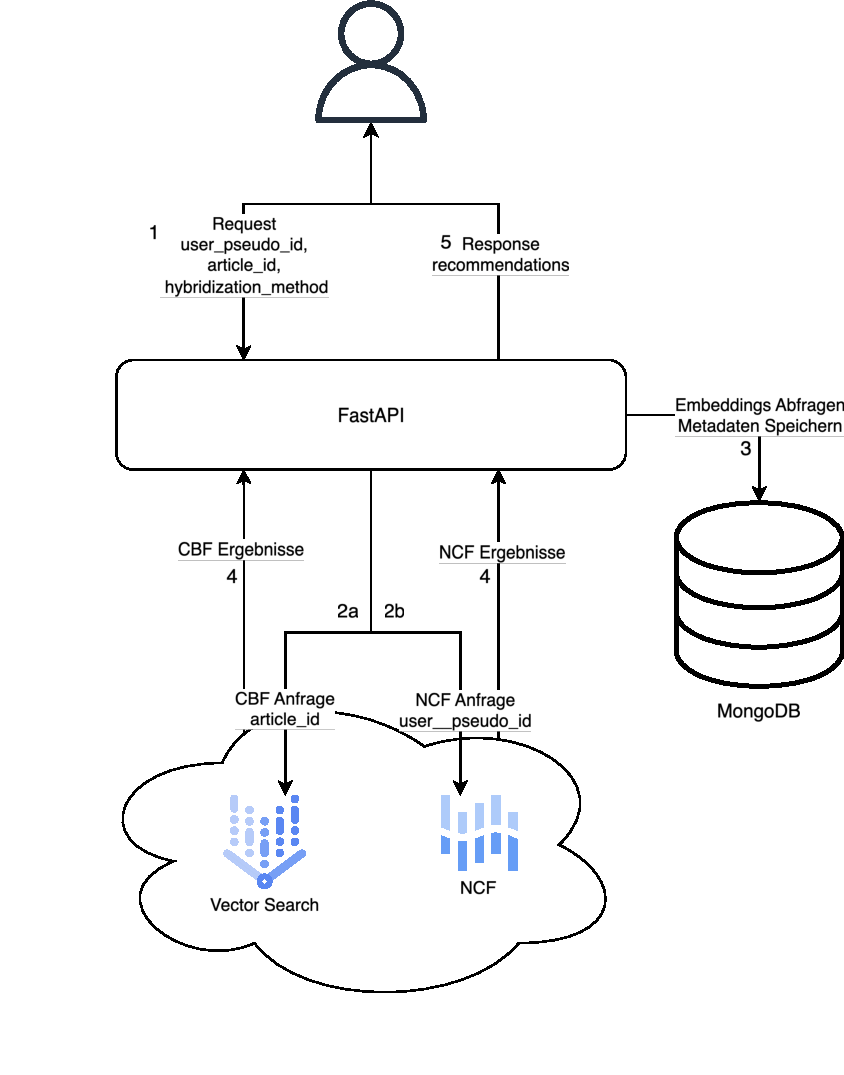
\includegraphics[width=0.6\textwidth]{content/figures/svg/architektur.pdf}
    \caption{Die technologische Architektur des hybriden Empfehlungssystems. Der nummerierte Datenfluss zeigt den Weg einer Anfrage vom Nutzer (1), 
    über die parallelen Abfragen an die ML-Dienste (2a, 2b) und die Datenbank (3), die eintreffenden Ergebnisse (4) bis zur finalen Empfehlung (5).}
    \label{fig:architektur}
\end{figure}
Die technologische Architektur ist als cloud-nativer Microservice-Ansatz auf der \ac{GCP} konzipiert,
um die in Abschnitt \ref{sec:nfr} definierten Anforderungen an Skalierbarkeit und Performanz zu erfüllen. 
Als zentraler Orchestrator dient ein in Python implementierter Service, der auf dem performanten FastAPI-Framework basiert. 
Dieser Service ist nicht nur für die Entgegennahme von Anfragen und die Steuerung der Modell-Endpunkte verantwortlich, 
sondern auch für die Hybridisierung der Empfehlungsergebnisse. Das Design wurde modular gestaltet, 
um zukünftig auch fortgeschrittenere Hybridisierungsstrategien integrieren zu können.

\subsubsection{API-Design und Orchestrierung}
\label{sec:api_design}

Das Herzstück des Systems bildet der API-Service, welcher die Schnittstelle nach außen darstellt und die interne Logik steuert. 
Die API wird über einen REST-Endpunkt unter der Adresse \texttt{/v1/recommendations} bereitgestellt und kommuniziert über einen 
JSON-basierten Datenvertrag. Eine Anfrage an den Dienst enthält die \texttt{user\_pseudo\_id}, die \texttt{article\_id} 
als Kontext sowie die gewünschte Hybridisierungsstrategie. 

Die Implementierung basiert auf dem Python-Framework FastAPI, das aufgrund seiner hohen asynchronen Leistungsfähigkeit durch das \ac{ASGI} und 
der automatischen Generierung interaktiver Dokumentation ausgewählt wurde. Der Service orchestriert bei 
jeder Anfrage die parallelen Abfragen an die untergeordneten ML-Dienste und die Datenbank, führt die Ergebnisse zusammen 
und wendet die Logik zur Hybridisierung an, bevor die finale Empfehlungsliste an den Client zurückgesendet wird.

\subsubsection{Content-Based Filtering mittels Vektorsuche}
\label{sec:cbf_service}

Die technische Umsetzung des \ac{CBF}-Ansatzes erfolgt mittels der Vertex AI Vektorsuche. 
Das Finden der thematisch ähnlichsten Artikel zu einem gegebenen Beitrag ist ein Nearest-Neighbor-Problem
im hochdimensionalen Vektorraum. 
Eine exakte Brute-Force-Suche über den gesamten Datenbestand ist für Echtzeitanwendungen mit geringer Latenz rechentechnisch nicht durchführbar.

Daher setzt Vertex AI Vektorsuche auf einen \ac{ANN}-Algorithmus. 
Dieser Ansatz tauscht eine geringfügige Einbuße an Genauigkeit gegen einen massiven Gewinn an Abfragegeschwindigkeit. 
Die zugrundeliegende Technologie ist Googles \ac{ScaNN}-Algorithmus, der im Kern auf zwei Prinzipien basiert:

\begin{itemize}
    \item \textbf{Partitionierung des Vektorraums:} Der Index unterteilt den hochdimensionalen Raum in eine Vielzahl von Clustern oder Zellen. 
    Bei einer Suchanfrage müssen dann nicht mehr alle Vektoren durchsucht werden, sondern nur noch die Vektoren in den wahrscheinlichsten Partitionen.
    \item \textbf{Vektorquantisierung:} Innerhalb dieser Partitionen werden die Vektoren durch eine Form der intelligenten Komprimierung repräsentiert, 
    um den Speicherbedarf zu reduzieren und Distanzberechnungen zu beschleunigen. Google setzt hierbei auf fortgeschrittene Methoden wie die anisotrope 
    Vektorquantisierung, um den Informationsverlust bei der Komprimierung zu minimieren \cite{avq_2020}.
\end{itemize}

Der ScaNN-Algorithmus lernt, die vielversprechendsten Partitionen für eine gegebene Anfrage effizient zu identifizieren und führt dann innerhalb 
dieser Partitionen eine schnelle Distanzberechnung auf den quantisierten Vektoren durch. 
Die Forschung zur Optimierung dieser Indexierungsstrategien entwickelt sich stetig weiter, wie das Paper zu SOAR zeigt, 
einem Nachfolger-Ansatz zur Verbesserung der Indexeffizienz \cite{soar_2023}.

\subsubsection{Neural Collaborative Filtering}
\label{sec:ncf_service}

Als kollaborativer Filteransatz wird in dieser Arbeit das \ac{NCF}-Modell eingesetzt. 
Traditionelle Ansätze wie die \ac{MF} modellieren die Interaktion zwischen Nutzern und Artikeln durch ein einfaches Skalarprodukt ihrer latenten Vektoren,
was die Ausdrucksstärke des Modells auf lineare Zusammenhänge limitiert.

Das NCF-Framework generalisiert diesen Ansatz, indem es das Skalarprodukt durch eine neuronale Architektur ersetzt. 
Konkret wird ein \ac{MLP} genutzt, um eine beliebige, auch nicht-lineare Interaktionsfunktion direkt aus den Daten zu erlernen \cite{he_neural_2017}. 
Diese Fähigkeit, komplexe Muster im Nutzer-Item-Interaktionsverhalten zu erfassen, macht das NCF-Modell zu einer 
leistungsfähigen Wahl für die Generierung personalisierter Empfehlungen.
Für den produktiven Einsatz wird das trainierte Modell auf einem dedizierten Vertex AI Endpoint bereitgestellt, 
um skalierbare Echtzeit-Inferenzen für gegebene Nutzer-IDs zu ermöglichen.

\subsection{Datenbasis und Einschränkungen}
\label{sec:data}
Der für das \ac{NCF}-Modell zugrundeliegende Datensatz SM-News-Jan25 bezieht sich ausschließlich auf \ac{GA4}-Daten vom Januar 2025.
Der Grund für diese Einschränkung liegt in den Kosten des Modelltrainings für große Datensätze. Für das Training werden die ersten drei Wochen 
und für den Test die letzte Woche des SM-News-Jan25 genutzt. 

Eine zentrale Eigenschaft des Datensatzes ist seine stark rechtsverschobene Verteilung, 
sowohl bei der Artikelpopularität als auch bei der Nutzeraktivität. Dieses als Long-Tail-Verteilung 
bekannte Phänomen ist typisch für Mediendaten und stellt eine Kernherausforderung für Empfehlungssysteme dar \cite{wu_personalized_2022, raza_news_2020}.

% content/figures/plot_artikelverteilung_train.tex

\begin{figure}[H]
    \centering
    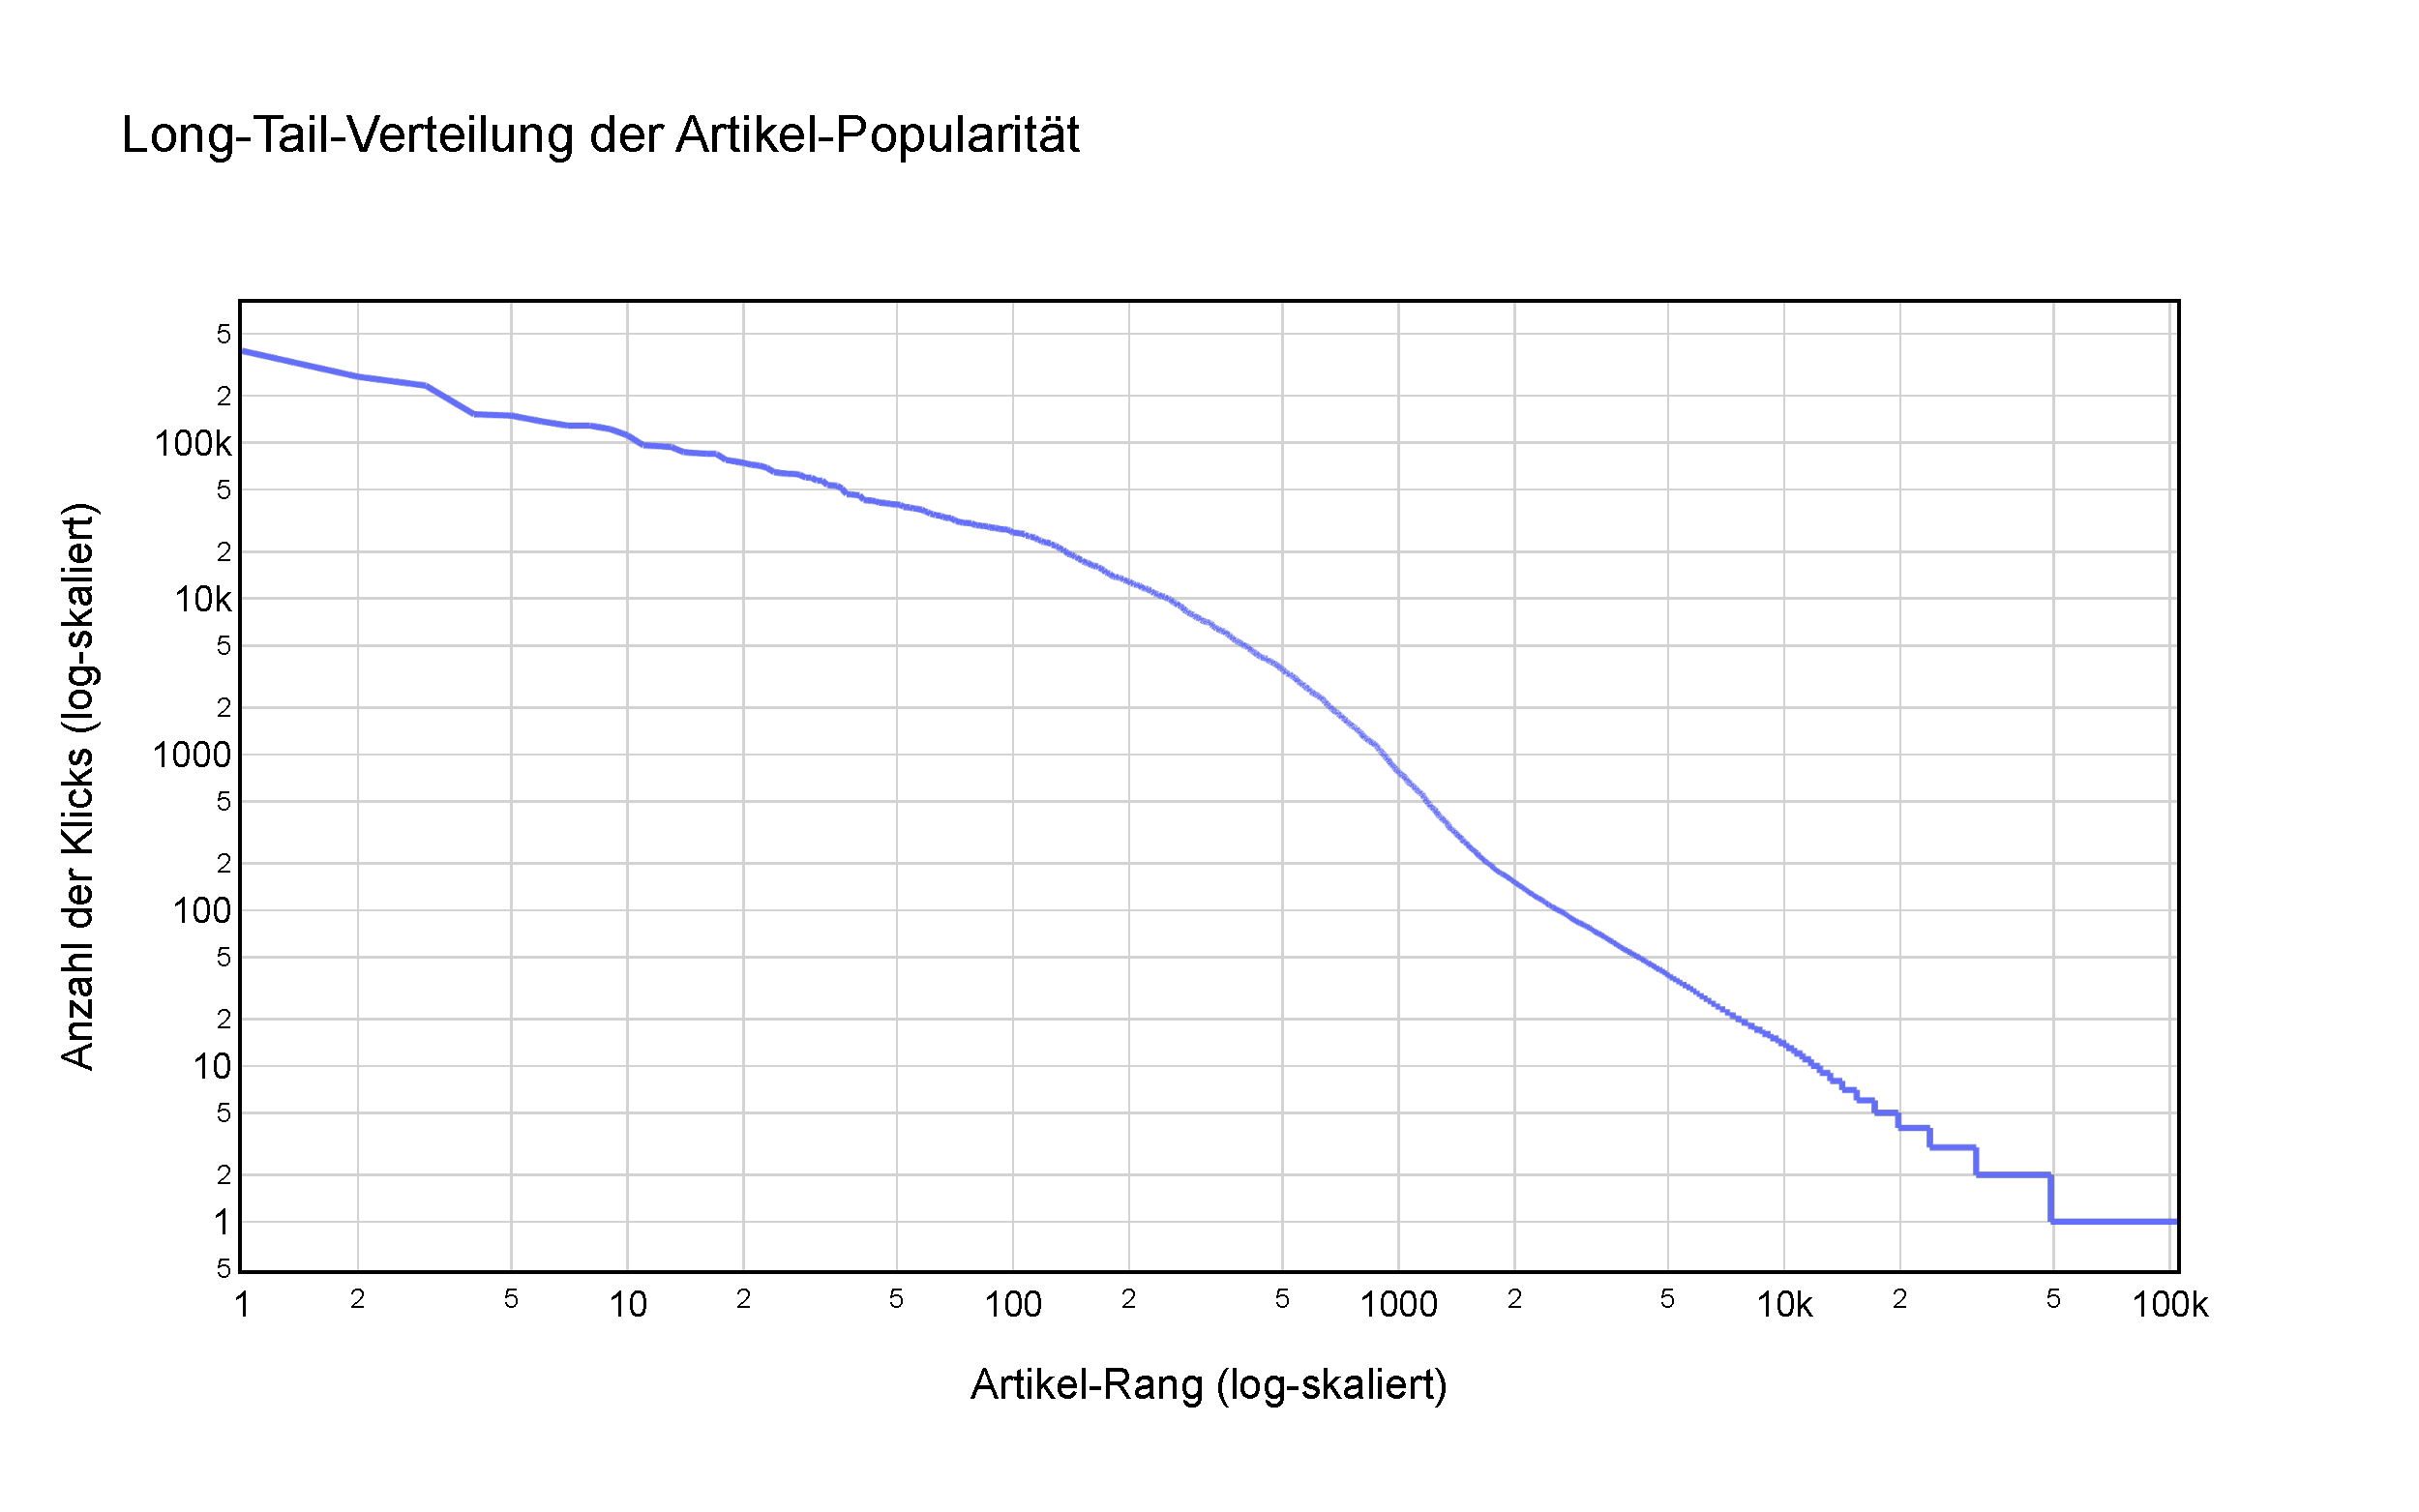
\includegraphics[width=0.9\textwidth]{content/figures/svg/artikel_verteilung_train.pdf}
    \caption{Popularitätsverteilung der Artikel im Trainingsdatensatz. Die Grafik zeigt, dass eine geringe Anzahl von Artikeln einen Großteil der Klicks auf sich vereint, während die Mehrheit der Artikel nur wenige Interaktionen erhält (Long-Tail).}
    \label{fig:artikelverteilung_train}
\end{figure}

Die Verteilung manifestiert sich in zwei Dimensionen:

\begin{itemize}
    \item 
    \textbf{Artikelpopularität:} Wie in Abbildung~\ref{fig:artikelverteilung_train} dargestellt,\newline 
    konzentriert sich ein 
    überproportional großer Anteil der Seitenaufrufe auf eine sehr kleine Gruppe von viralen "Hit"-Artikeln, die den "Kopf" der Verteilung bilden. 
    Dies wird durch die kurze Lebensdauer von Nachrichtenartikeln zusätzlich verstärkt.
    \item \textbf{Nutzeraktivität:} Ein analoges Muster zeigt sich beim Nutzerverhalten. 
    Eine kleine Kohorte von hochaktiven "Power-Nutzern" ist für einen Großteil der Klick-Events verantwortlich, während die Mehrheit der Nutzer nur 
    sporadisch mit wenigen Klicks interagiert.
\end{itemize}

Diese ungleiche Verteilung führt zu einem inhärenten Popularity Bias in den Daten. 
Naive Modelle neigen dazu, allen Nutzern wiederholt dieselben populären Bestseller-Artikel zu empfehlen, 
was das Ziel der Personalisierung untergräbt und die Gefahr birgt, Nutzer in einer Filterblase zu isolieren. 
Gleichzeitig entsteht ein Kaltstart-Problem für Nischen-Artikel im Long Tail, die kaum eine Chance haben, empfohlen zu werden. 
Eine zentrale Herausforderung dieser Arbeit ist daher die Konzeption eines Systems, 
das diesen Popularity Bias aktiv ausbalanciert, um auch relevante Nischeninhalte an die passenden Nutzer auszuspielen.

% content/figures/plot_nutzerverteilung_train.tex

\begin{figure}[H]
    \centering
    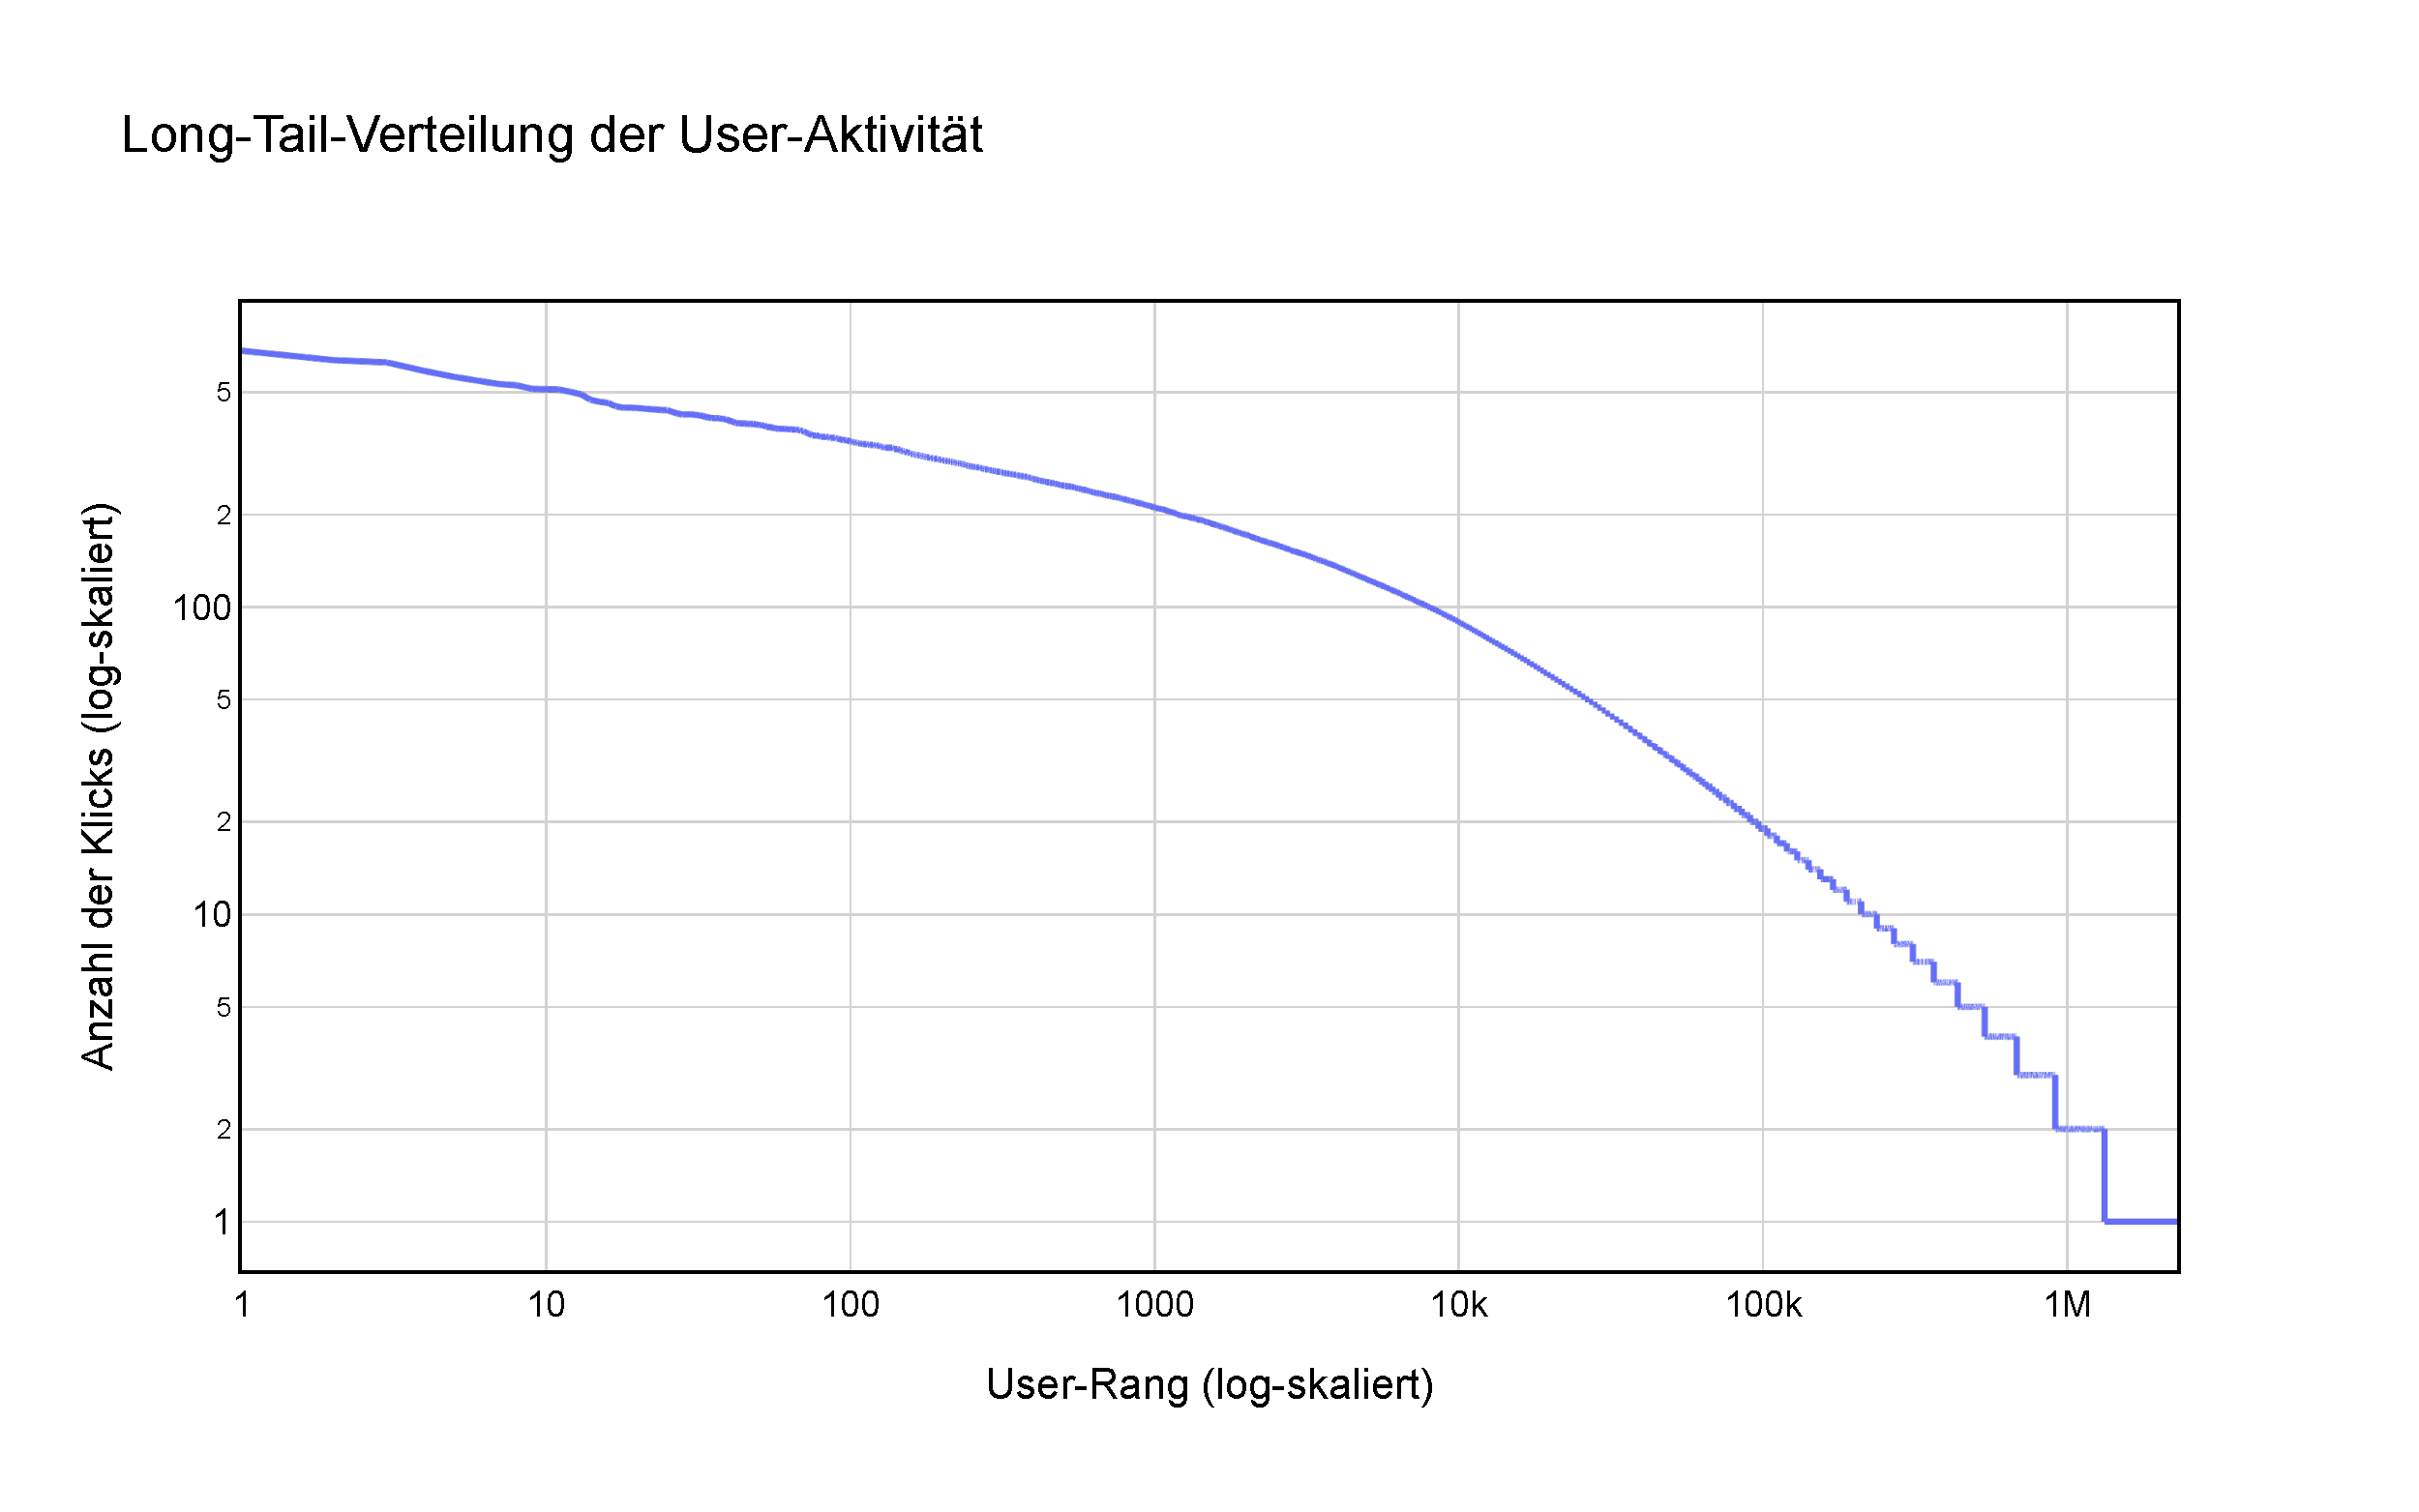
\includegraphics[width=0.9\textwidth]{content/figures/svg/nutzer_verteilung_train.pdf}
    \caption{Verteilung der Nutzeraktivität im Trainingsdatensatz. Die Darstellung verdeutlicht die typische Long-Tail-Verteilung: Eine große Anzahl von Nutzern interagiert nur selten mit Artikeln, während eine kleine Gruppe von "Power-Nutzern" für einen Großteil der Klicks verantwortlich ist.}
    \label{fig:nutzerverteilung_train}
\end{figure}

Die zugrundeliegenden statistischen Kennzahlen des Trainingsdatensatzes sind in Tabelle~\ref{tab:train_stats} zusammengefasst.

% content/tables/statistiken_trainingsdaten.tex

\begin{table}[H]
    \centering
    \caption{Statistische Kennzahlen des Trainingsdatensatzes, basierend auf den Klick-Logs der ersten drei Januarwochen.}
    \label{tab:statistiken_training}
    \begin{tabular}{lr}
        \toprule
        \textbf{Metrik} & \textbf{Wert} \\
        \midrule
        Gesamte Interaktionen (Klicks) & 11.412.116 \\
        Einzigartige user\_pseudo\_ids & 2.294.733 \\
        Einzigartige Artikel & 104.462 \\
        \bottomrule
    \end{tabular}
\end{table}
\label{tab:train_stats}

Um die Klick-Events für das \ac{NCF}-Modell nutzbar zu machen, wurden sie in eine User-Item-Interaktionsmatrix überführt. 
Dabei repräsentieren die Zeilen die einzigartigen Nutzer und die Spalten die einzigartigen Artikel des Trainingszeitraums. 
Eine Zelle $(i, j)$ in der Matrix erhält den Wert 1, wenn der Nutzer $i$ mit dem Artikel $j$ interagiert hat, andernfalls den Wert 0. 
Dieser Prozess resultiert in einer binären Matrix, die das implizite Feedback der Nutzer abbildet.

\newpage
Die resultierende Matrix weist mit Dimensionen von circa 2,3 Millionen Nutzern und 104.000 Artikeln eine Dichte von unter 0,005\,\% auf. 
Ihre entscheidende Eigenschaft ist daher ihre extreme Dünnbesetzung. 
Diese Sparsity ist eine typische Herausforderung für \ac{CF}-Modelle, da für jeden Nutzer nur eine verschwindend geringe Anzahl an Interaktionen im Verhältnis zur Gesamtmenge der Artikel vorliegt. 
Dies erschwert es dem Modell, aussagekräftige Muster im Nutzerverhalten zu erlernen und auf neue User-Item-Paare zu generalisieren.

Bei der Interpretation der Ergebnisse müssen folgende Limitationen berücksichtigt werden:

\begin{itemize}
    \item \textbf{Zeitlicher Rahmen:} Der verwendete Datensatz deckt ausschließlich den Januar 2025 ab. 
    Dies stellt eine Momentaufnahme dar und verhindert, dass das Modell saisonale Effekte (z.B. Feiertage) oder langfristige Entwicklungen im Nutzerinteresse erfassen kann.

    \item \textbf{Implizites Feedback:} Als Interaktionssignal werden ausschließlich Klicks verwendet. 
    Diese Form des impliziten Feedbacks ist zwar reichlich vorhanden, aber mehrdeutig. 
    Ein Klick ist kein garantierter Indikator für Nutzerzufriedenheit; er kann auch zu einem sofortigen Verlassen der Seite (Bounce) führen. 
    Andere Signale wie die Verweildauer wurden in diesem Prototypen nicht berücksichtigt.

    \item \textbf{Offline-Evaluation:} Die Modellgüte wird offline anhand historischer Daten mit Metriken wie dem \ac{nDCG} evaluiert. 
    Diese Methodik kann die tatsächliche Auswirkung auf das Nutzerverhalten im Live-Betrieb nicht vollständig abbilden. 
    Um den realen Business Impact auf KPIs wie Sitzungsdauer oder Nutzerbindung zu messen, wäre ein abschließender Online-A/B-Test der nächste logische Schritt.
\end{itemize}

\section{Optimierung der Empfehlungsqualität}
\label{chap:opt}
% V-Ansatz Teil 3 – Evaluation und Optimierung

% TODO: NDCG@10 Skalen der Abbildungen vereinheitlichen

\subsection{Zielfunktion}
\label{sec:target_function}
Als Zielfunktion für die Optimierung des hybriden Empfehlungssystems dient eine gewichtete 
Linearkombination der Scores der beiden zugrundeliegenden Modelle. Dieser Ansatz wurde 
aufgrund seiner einfachen Interpretierbarkeit und seiner weiten Verbreitung als robuste 
Baseline für hybride Architekturen gewählt (vgl. \cite{burke_hybrid_2002}). 
Die mathematische Formulierung der Funktion lautet:

\begin{equation}
\label{eq:target}
s_\mathrm{hybrid} = w_\mathrm{cbf} \cdot s_\mathrm{cbf} + w_\mathrm{cf} \cdot s_\mathrm{cf}
\end{equation}

Die einzelnen Terme der Gleichung sind wie folgt definiert:
\begin{itemize}
    \item $s_\mathrm{hybrid}$: Der finale, kombinierte Score für ein potenziell zu empfehlendes Item. 
    Die finale Empfehlungsliste wird durch das absteigende Sortieren der Items nach diesem Score erstellt.
    
    \item $s_\mathrm{cbf}$ und $s_\mathrm{cf}$: Die von der Content-Based- bzw. der Collaborative-Filtering-Komponente 
    generierten Roh-Scores. Vor der Kombination in der Zielfunktion ist eine Normalisierung dieser 
    Scores erforderlich, um sicherzustellen, dass sie auf einer vergleichbaren Skala liegen.
    In dieser Arbeit werden die Scores mit der Min-Max-Skalierung auf $[0, 1]$ normalisiert.
    
    \item $w_\mathrm{cbf}$ und $w_\mathrm{cf}$: Die nicht-negativen Gewichtungsparameter, welche den Einfluss 
    der jeweiligen Modellkomponente auf das Endergebnis steuern. Für diese Gewichte gilt die Nebenbedingung 
    $w_\mathrm{cbf} + w_\mathrm{cf} = 1$, wodurch die Optimierung auf die Bestimmung eines einzigen 
    Parameters reduziert wird.
\end{itemize}

Das zentrale Ziel des in~\ref{sec:opt_strat} beschriebenen Optimierungsprozesses 
ist es, die optimalen Werte für die Gewichtungsparameter $w_\mathrm{cbf}$ und $w_\mathrm{cf}$ zu finden, 
sodass die in Abschnitt~\ref{sec:metrics} definierte Evaluationsmetrik (nDCG@10) maximiert wird.

\subsection{Evaluationsmetriken}
\label{sec:metrics}
Die empirische Bewertung und Optimierung des hybriden Empfehlungssystems erfordert ein klar definiertes 
Evaluationsprotokoll sowie eine geeignete Zielfunktion. Als primäre Zielfunktion für die in Kapitel 4 
beschriebene Hyperparameter-Optimierung dient die Maximierung der Empfehlungsqualität, gemessen durch 
den normalisierten diskontierten kumulativen Gewinn bei einer Listenlänge von 10 (nDCG@10). Diese Metrik 
wurde ausgewählt, da sie nicht nur die reine Trefferquote erfasst, sondern vor allem die exakte Position 
eines relevanten Treffers innerhalb der Empfehlungsliste gewichtet, was das reale Nutzerverhalten präzise abbildet.

Die besondere Eignung des nDCG als Metrik für Empfehlungssysteme liegt in seiner positions-sensitiven 
("top-heavy") Natur. Mathematisch wird dies durch eine logarithmische Diskontierung erreicht, bei der der 
Wert eines Treffers am Rang $r$ mit dem Faktor $1/\log_2(r+1)$ abgewertet wird. Dies führt dazu, dass ein 
Treffer an den vordersten Rängen überproportional mehr zur Gesamtbewertung beiträgt als ein Treffer an einer 
späteren Position. So ist beispielsweise ein relevanter Artikel an Rang 1 signifikant wertvoller als 
an Rang 2, während der Unterschied zwischen Rang 100 und 101 nur noch marginal ist. Diese Eigenschaft ist 
essenziell, da Nutzer Interaktionen auf den vordersten Plätzen der Ergebnisliste konzentrieren und weiter 
hinten platzierte Vorschläge selten beachten (vgl. \cite{krichene_sampled_2020}).

Ein entscheidender Aspekt des Evaluationsdesigns ist die Handhabung negativer Instanzen. Anstatt auf 
Verfahren des Negative Samplings zurückzugreifen, bei denen eine kleine, zufällige Teilmenge 
nicht-interagierter Artikel als negative Beispiele dient, wird in dieser Arbeit eine 
methodisch rigorosere Strategie des \textit{Full-Catalog Rankings} verfolgt. Bei diesem Vorgehen muss 
das Modell für jeden positiven Testfall den relevanten Artikel aus der Gesamtheit aller im 
Datensatz verfügbaren Artikel – abzüglich der bereits vom Nutzer gelesenen – identifizieren.

Diese Methode vermeidet systematische Verzerrungen (sampling bias), die durch ein 
unausgewogenes Sampling entstehen können, und simuliert ein anspruchsvolles, aber realistisches 
Anwendungsszenario. Die Evaluation auf dem gesamten Artikelkatalog stellt eine enorme 
Herausforderung für das Empfehlungssystem dar, was naturgemäß zu absolut gesehen niedrigen 
Metrikwerten führt. Wie in der Fachliteratur bestätigt wird, sind solche Ergebnisse jedoch nicht 
als Indikator für eine geringe Modellleistung zu interpretieren, sondern als Konsequenz eines 
besonders anspruchsvollen und unverzerrten Evaluationsprotokolls 
(vgl. \cite{krichene_sampled_2020}). Die auf diese Weise gewonnenen Erkenntnisse bieten eine 
robuste und verlässliche Grundlage für die zukünftige Weiterentwicklung von 
Empfehlungssystemen bei der SV-Gruppe.

\subsection{Experimenteller Aufbau und Validierungsdatensatz}
Die Grundlage für die Optimierung und Evaluation bildet ein Validierungsdatensatz, der aus den 
Nutzerinteraktionen der letzten Januarwoche 2025 extrahiert wurde. Die statistischen Kennzahlen 
dieses Zeitraums sind in Tabelle~\ref{tab:statistiken_test} zusammengefasst.

% content/tables/statistiken_testdaten.tex

\begin{table}[htbp]
    \centering
    \caption{Statistische Kennzahlen des Test- und Validierungsdatensatzes, basierend auf den Klick-Logs der letzten Januarwoche.}
    \label{tab:statistiken_test}
    \begin{tabular}{lr}
        \toprule
        \textbf{Metrik} & \textbf{Wert} \\
        \midrule
        Gesamte Artikelaufrufe & 3.627.024 \\
        Einzigartige user\_pseudo\_ids & 1.099.289 \\
        Einzigartige Artikel & 57.100 \\
        \bottomrule
    \end{tabular}
\end{table}

Aus dem Gesamt-Pool an Nutzern wurde eine repräsentative Validierungsstichprobe von 1.000 
einzigartigen Nutzern zufällig gezogen, um den für die Optimierung erforderlichen Rechenaufwand in einem praktikablen 
Rahmen zu halten. Für jeden Nutzer in der Stichprobe wurde nach dem \textit{Leave-Last-Out}-Prinzip 
der letzte interagierte Artikel als Ground Truth für die Evaluation definiert (vgl. \Cite{Rendle_BPR_2009}).

\subsection{Optimierungsstrategie}
\label{sec:opt_strat}
Die Bestimmung der optimalen Gewichtungsparameter $w_\mathrm{cbf}$ und $w_\mathrm{cf}$ aus 
Gleichung~\ref{eq:target} erfolgt durch einen automatisierten Hyperparameter-Optimierungsprozess.

Als Framework für diesen Prozess wurde \textit{Optuna} (\Cite{Akiba_Optuna_2019}) gewählt, das eine effiziente Suche im 
Parameterraum ermöglicht. Über insgesamt 515 Iterationen (Trials) wurden verschiedene 
Gewichtungskombinationen evaluiert, mit dem Ziel, die in Abschnitt~\ref{sec:metrics} definierte 
nDCG@10-Metrik zu maximieren.

Der Ablauf eines einzelnen Optimierungs-Trials gestaltet sich wie folgt:
\begin{enumerate}
    \item Optuna schlägt eine neue Wertekombination für $w_\mathrm{cbf}$ und $w_\mathrm{cf}$ vor.
    \item Für jeden der 1.000 Nutzer in der Validierungsstichprobe werden die Empfehlungen der 
    \ac{CBF}- und \ac{CF}-Modelle über deren jeweilige API-Endpunkte parallel und asynchron abgerufen.
    \item Die Ergebnislisten der beiden Modelle werden mittels der vorgeschlagenen Gewichte zu einer 
    finalen hybriden Empfehlungsliste fusioniert.
    \item Der nDCG@10-Wert dieser finalen Liste wird berechnet, indem sie mit dem Ground-Truth-Artikel 
    des Nutzers verglichen wird.
    \item Der über alle 1.000 Nutzer gemittelte nDCG@10-Wert wird an Optuna zurückgegeben, um 
    den nächsten, informierteren Suchschritt zu steuern.
\end{enumerate}

Dieser Prozess entspricht einem Gesamtaufwand von 515.000 individuellen Evaluierungen des 
Hybridmodells, was eine gründliche und robuste Suche nach der optimalen Parameterkonfiguration 
gewährleistet.

Die Visualisierung der Optimierungslandschaft in Abbildung~\ref{fig:hyperparameterraum} verdeutlicht die 
komplexe, nicht-lineare Beziehung zwischen den Modellgewichten und der resultierenden Empfehlungsqualität. 
Angesichts dieser zerklüfteten Landschaft mit mehreren lokalen Optima ist ein naiver Ansatz wie eine 
Rastersuche (Grid Search) ineffizient. Der Einsatz eines fortschrittlichen Optimierungsframeworks 
wie Optuna, das mit intelligenten Suchalgorithmen arbeitet, ist daher notwendig, um den global 
optimalen Bereich im Parameterraum effizient und verlässlich zu identifizieren.

% content/figures/plot_hyperparameterraum.tex

\begin{figure}[H]
    \centering
    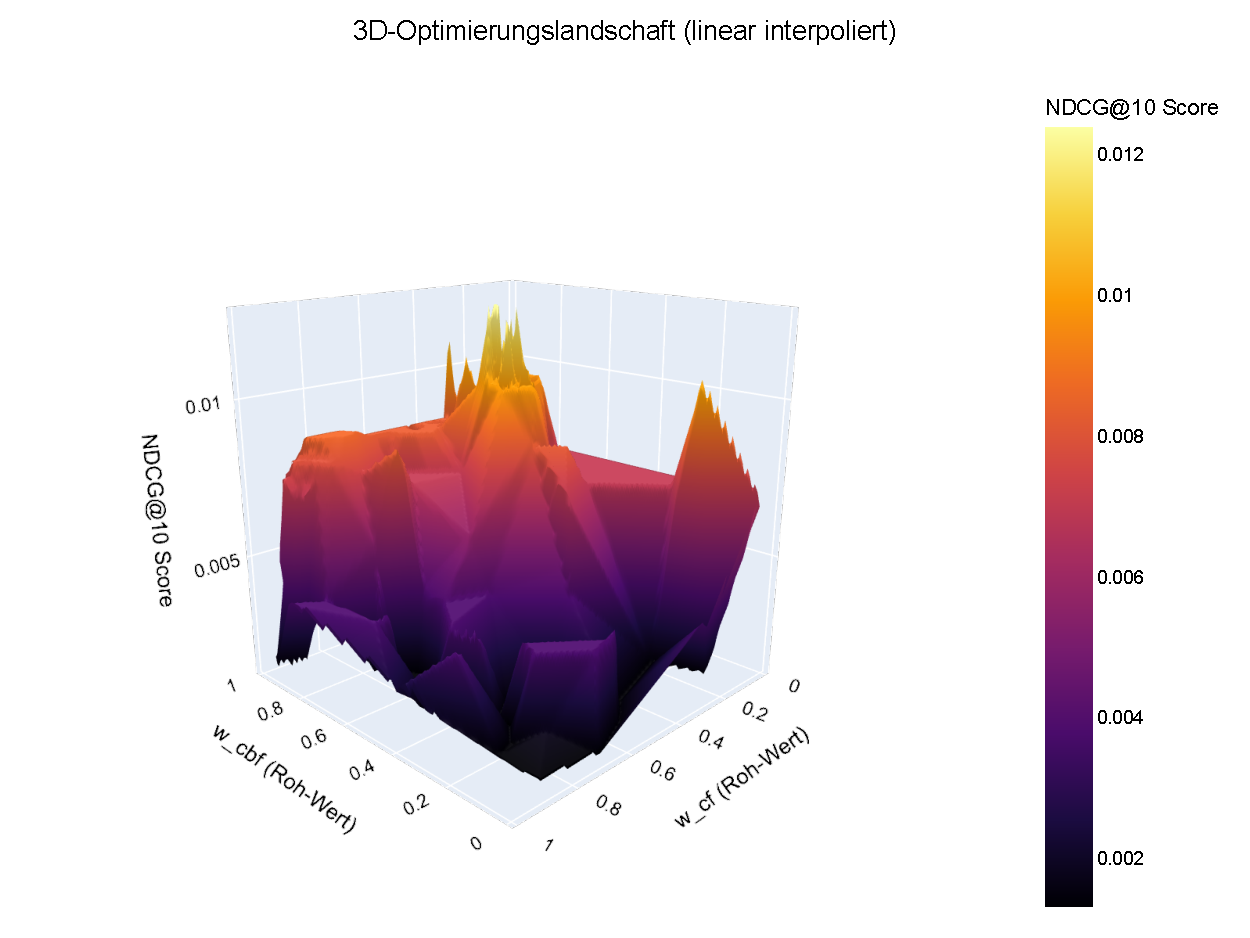
\includegraphics[width=0.9\textwidth]{content/figures/svg/hyperparameterraum.pdf}
    \caption{Visualisierung des zweidimensionalen Hyperparameterraums der Modellgewichtungen. Die Achsen repräsentieren die Gewichte für das CBF-Modell (\(w_{cbf}\)) und das CF-Modell (\(w_{cf}\)). Die Einfärbung der Punkte visualisiert den resultierenden NDCG@10-Wert für jede Konfiguration aus dem Optuna-Suchlauf.}
    \label{fig:hyperparameterraum}
\end{figure}

Konkret wurde für die Suche der in Optuna standardmäßig implementierte \ac{TPE} als Suchalgorithmus verwendet (vgl. \cite{Akiba_Optuna_2019}). Der TPE-Algorithmus ist eine 
Variante der Bayes'schen Optimierung, die ein probabilistisches Modell der Zielfunktion erstellt, 
um intelligent zu entscheiden, welche Parameterkombination als Nächstes getestet werden soll. 
Dafür werden die bisherigen Evaluationsergebnisse in eine Gruppe mit vielversprechenden
und eine mit weniger erfolgreichen Ergebnissen aufgeteilt.

Für beide Gruppen werden separate Wahrscheinlichkeitsverteilungen modelliert. Der Algorithmus maximiert 
anschließend die erwartete Verbesserung Expected Improvement, indem er gezielt nach Parametern sucht, 
die eine hohe Wahrscheinlichkeit unter der Verteilung der guten Ergebnisse und gleichzeitig eine 
niedrige Wahrscheinlichkeit unter der Verteilung der schlechten Ergebnisse aufweisen. Diese Strategie 
ermöglicht eine effiziente Balance zwischen der Exploitation bereits bekannter guter 
Regionen und der Exploration neuer, potenziell noch besserer Bereiche des Suchraums. 
Durch diesen informierten Suchprozess kann das Optimum in komplexen Landschaften, wie der in 
Abbildung~\ref{fig:hyperparameterraum} gezeigten, deutlich schneller und ressourcenschonender 
gefunden werden als durch uninformierte Methoden.

\subsection{Ergebnisse}
\label{sec:results}
Der in Abschnitt~\ref{sec:opt_strat} beschriebene Optimierungsprozess führte zur Identifikation 
einer robusten Gewichtungskonfiguration für das hybride Empfehlungssystem. Die finale 
Evaluation zeigt, dass das optimierte Hybrid-Modell die definierten Baseline-Modelle 
in allen Metriken signifikant übertrifft.

Tabelle~\ref{tab:baseline_vergleich} listet die detaillierten Performance-Werte der evaluierten 
Modellvarianten auf, während Abbildung~\ref{fig:model_vergleich} eine visuelle 
Gegenüberstellung der Ergebnisse bietet.

% Inhalt von: content/tables/vergleich_baselines.tex

\begin{table}[htbp]
    \centering
    \caption{Vergleich des optimierten Hybrid-Modells mit den Baseline-Modellen anhand der Metriken NDCG@10 und Hit Rate@10.}
    \label{tab:baseline_vergleich}
    \begin{tabular}{lrr}
        \toprule
        \textbf{Modell} & \textbf{NDCG@10} & \textbf{Hit Rate@10} \\
        \midrule
        Unser Hybrid-Modell (Final) & 1.25\% & 1.8\% \\
        Popularity-Baseline        & 0.23\% & 0.6\% \\
        Recency-Baseline           & 0.14\% & 0.4\% \\
        \bottomrule
    \end{tabular}
\end{table}

% content/figures/vergleich_baselines.tex

\begin{figure}[H]
    \centering
    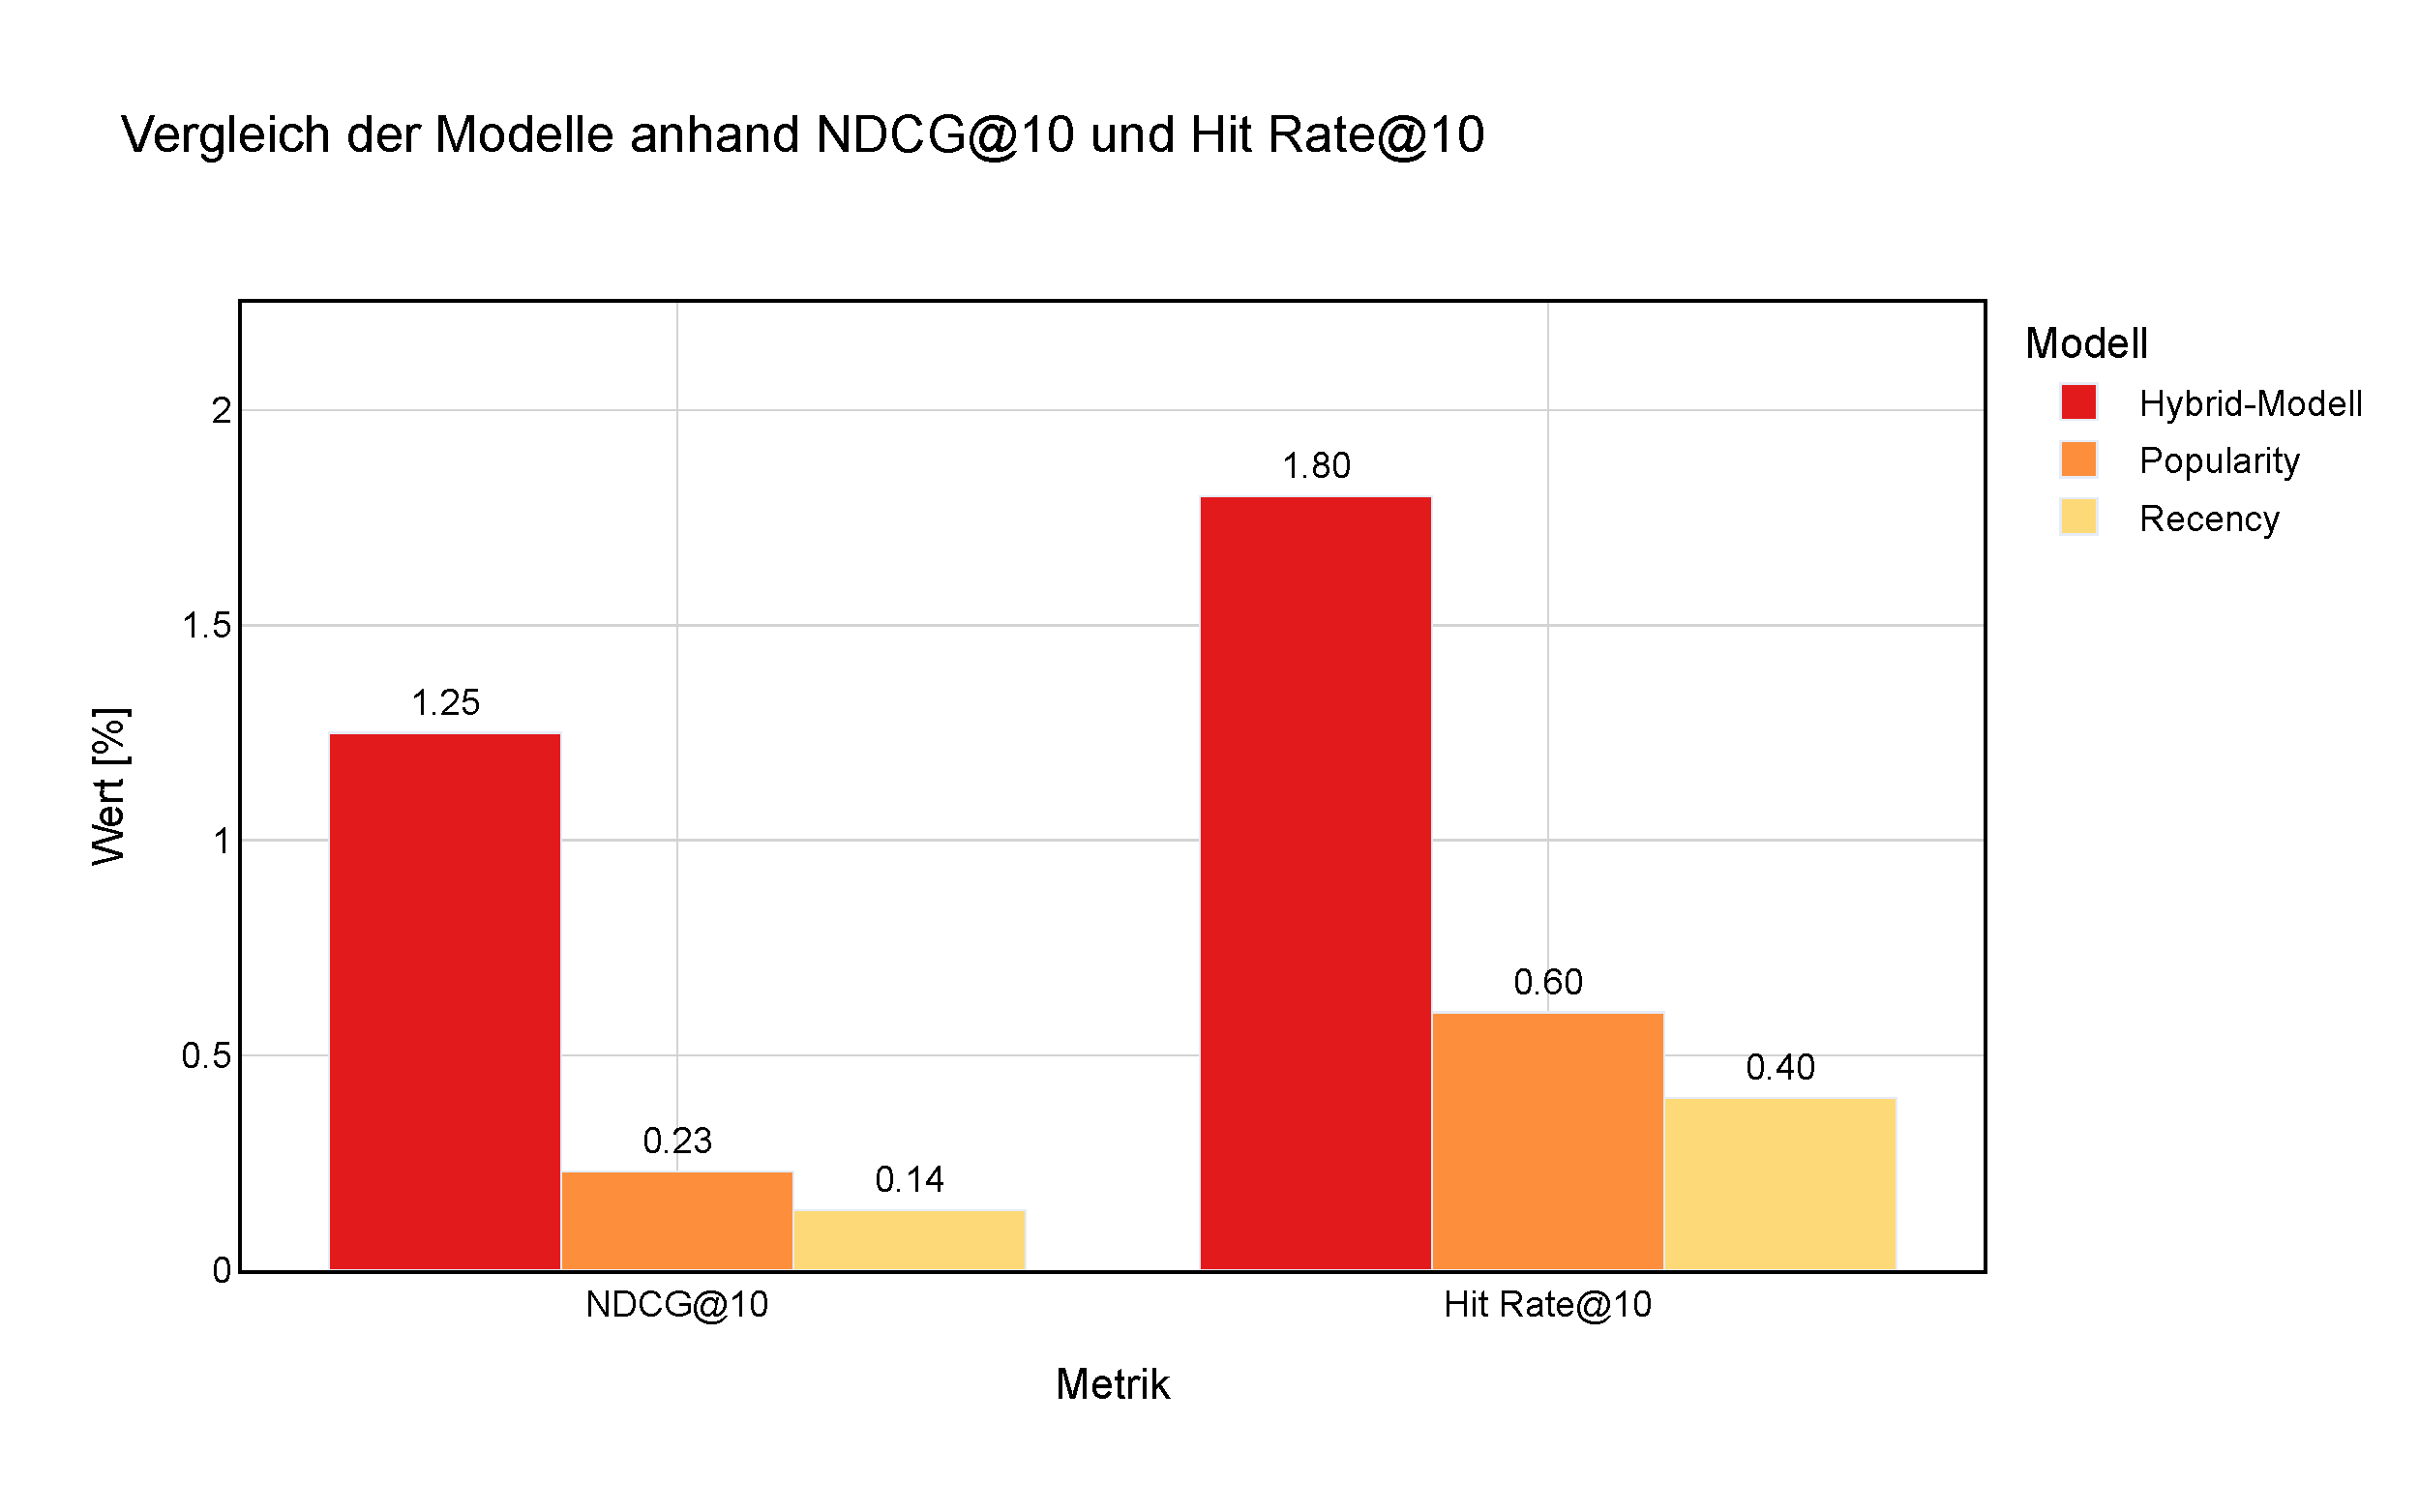
\includegraphics[width=0.8\textwidth]{content/figures/svg/model_baseline_comparison.pdf}
    \caption{Vergleich des Hybrid-Modells mit den Popularity- und Recency-Baselines anhand der Metriken NDCG@10 und Hit Rate@10.}
    \label{fig:model_vergleich}
\end{figure}

Abbildung~\ref{fig:kontourplot} zeigt die einzelnen Trials (Schwarze Punkte) auf der Hyperparameterlandschaft. 
Es ist gut zu erkennen, dass die größte Anzahl an optima in einem Bereich liegt, in dem $w_{cbf}$ größer als 0.5 ist und
$w_{cf}$ kleiner als 0.5.

Diese Ergebnisse bestätigen nicht nur die Wirksamkeit des gwählten
Hybridisierungsansatzes, sondern liefern auch den empirischen Beleg für dessen Überlegenheit gegenüber den reinen
Einzelkomponenten. Der Optimierungsprozess durchsuchte den gesamten Gewichtungsraum, einschließlich der Extremfälle,
die einem reinen \ac{CF}-Modell ($w_{cf} = 1$) oder einem reinen \ac{CBF}-Modell ($w_{cb} = 1$) entsprechen.
% content/figures/plot_kontour.tex

\begin{figure}[htbp]
    \centering
    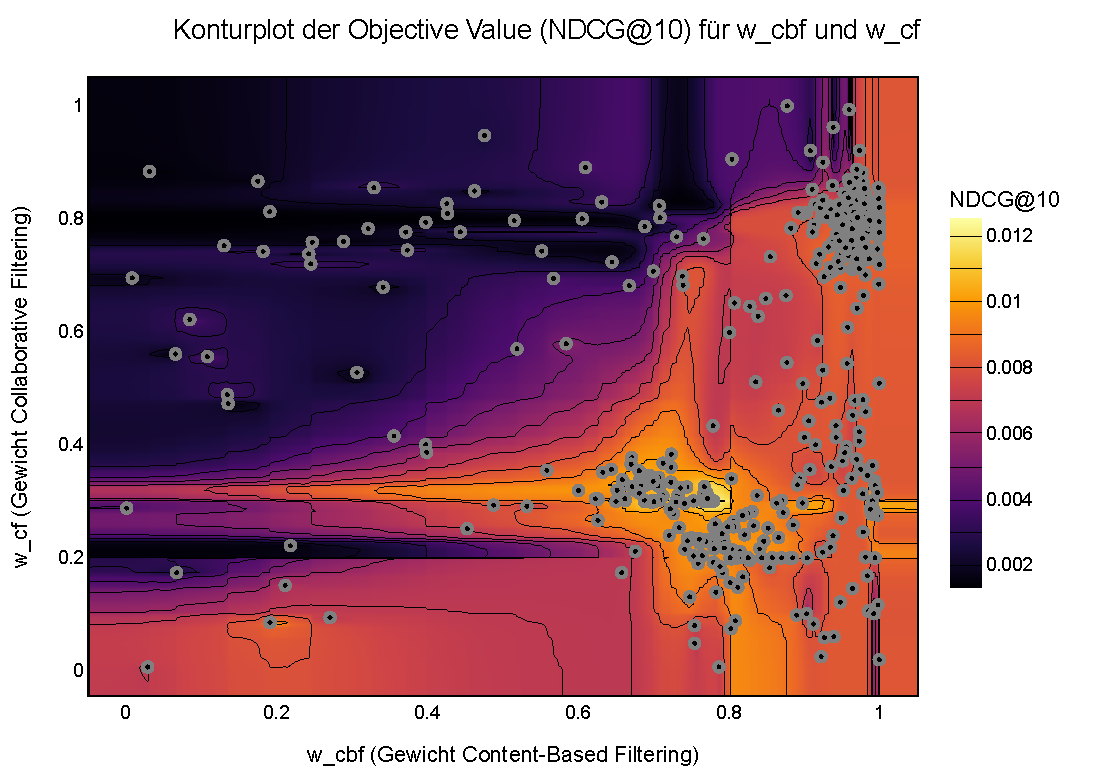
\includegraphics[width=0.9\textwidth]{content/figures/svg/kontourplot.pdf}
    \caption{Konturplot zur Darstellung der NDCG@10-Verteilung im zweidimensionalen Parameterraum der Modellgewichtungen. Die Isolinien verbinden Bereiche mit ähnlicher Performance.}
    \label{fig:kontourplot}
\end{figure}
Das identifizierte Optimum liegt jedoch klar bei einer Konfiguration von \(w_{cbf} \approx 0.7226\) und
\(w_{cf} \approx 0.2774\). Diese Tatsache belegt, dass beide Komponenten einen positiven Beitrag zur Maximierung
des \ac{nDCG}@10 leisten und die gewichtete Kombination eine signifikant höhere Empfehlungsqualität erzielt, als es durch den
alleinigen Einsatz des \ac{CBF}- oder \ac{CF}-Modells möglich gewesen wäre. Die konzeptionelle Notwendigkeit des hybriden
Ansatzes zur Ausbalancierung von Relevanz und Diversität wird somit durch die datengetriebene Optimierung quantitativ
untermauert.

Die dominante Rolle der \ac{CBF}-Komponente wird in Abbildung~\ref{fig:2d_performance} nochmals verdeutlicht. Die 
Visualisierung zeigt die \ac{nDCG}@10 Performance aller 515 Trialsin Abhängigkeit vom normalisierten \ac{CBF}-Gewicht.

Es ist ein deutlicher Leistungssprung (Phasensprung) bei einem Gewicht von \(w_{cbf} \approx 0.5\) zu erkennen.
Unterhalb dieser Schwelle werden durchweg nur niedrige \ac{nDCG}@10-Werte erreicht. Oberhalb davon steigt die Performance 
signifikant an, und alle optimalen Ergebnisse (orange markiert) konzentrieren sich im Bereich \(w_{cbf} > 0.6\)

Diese Beobachtung untermauert die Hypothese, dass im Nachrichtenkontext der unmittelbare thematische Bezug zum 
gerade gelesenen Artikel der stärkste Prädiktor für die nächste Interaktion ist. 
Das CBF-Modell liefert hier das notwendige Fundament für eine relevante Empfehlung. 
Die CF-Komponente dient in diesem Zusammenspiel als entscheidender „Fein-Tuner”, der auf dieser starken Basis aufsetzt, 
um die Performance durch Personalisierung auf das globale Maximum zu heben, wie es im Konturplot (Abbildung~\ref{fig:kontourplot}) 
ersichtlich wurde.

% content/figures/plot_2d_performance.tex

\begin{figure}[H]
    \centering
    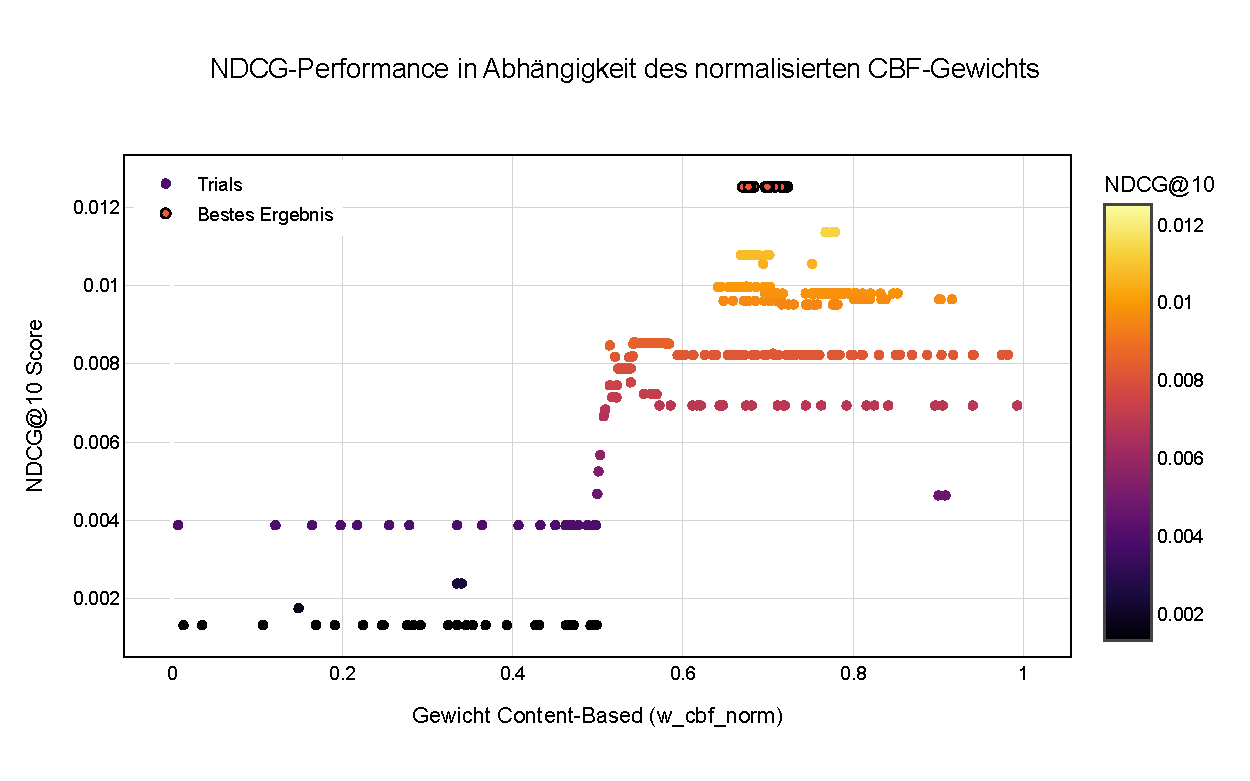
\includegraphics[width=0.9\textwidth]{content/figures/svg/2d_performance.pdf}
    \caption{2D-Darstellung des Hyperparameterraums. Die Achsen zeigen die Gewichtungen für das CBF- (\(w_{cbf}\)) und CF-Modell (\(w_{cf}\)). Die Farbe der Punkte indiziert den erreichten NDCG@10-Score. Der optimale Punkt ist markiert.}
    \label{fig:2d_performance}
\end{figure}
% % content/figures/plot_3d_scatter.tex

\begin{figure}[htbp]
    \centering
    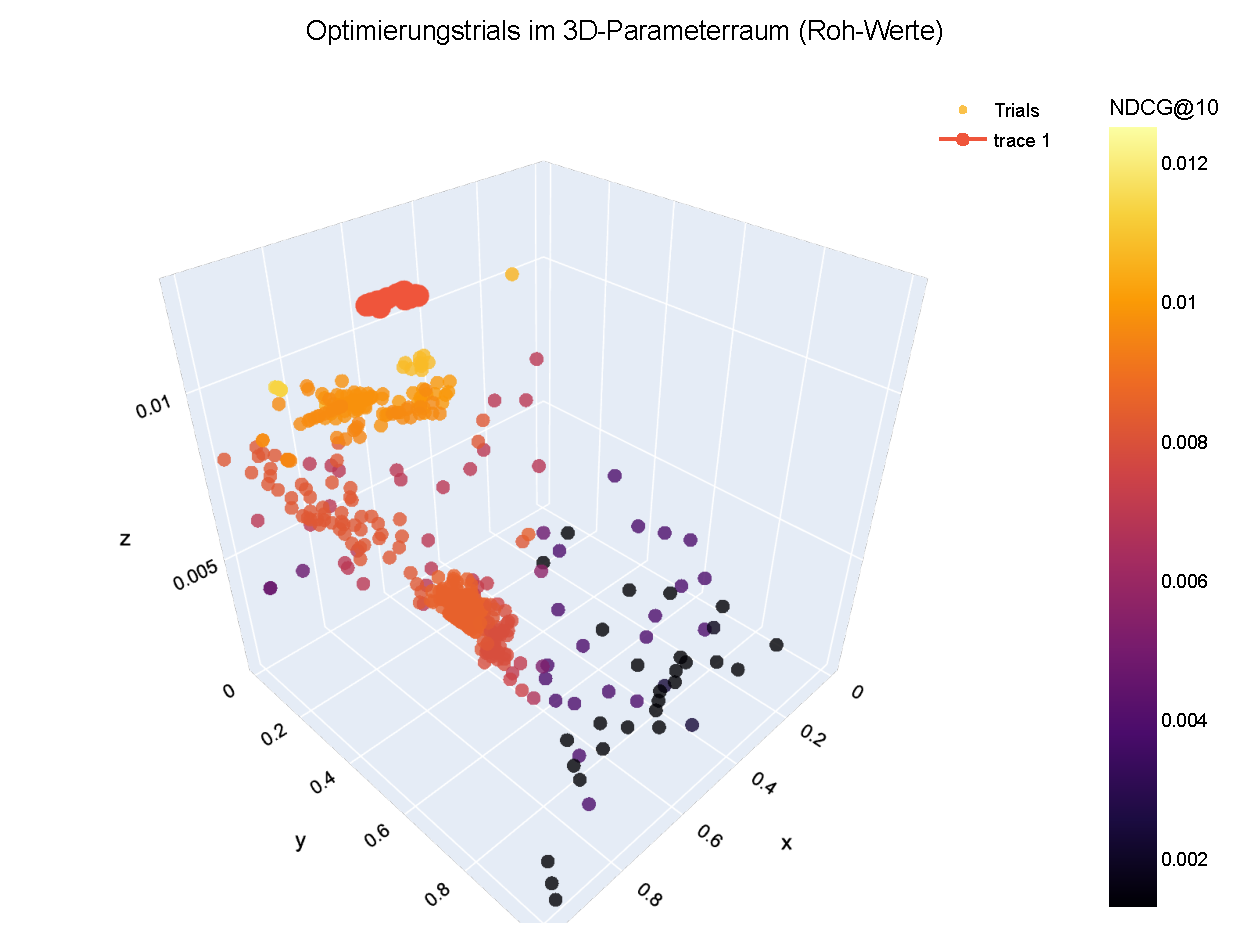
\includegraphics[width=0.8\textwidth]{content/figures/svg/3d_scatter_plot.pdf}
    \caption{Interaktives 3D-Streudiagramm der Optuna-Trials zur Visualisierung der Parameterabhängigkeiten. (Hinweis: Die Darstellung in der PDF-Version der Arbeit ist eine statische Ansicht).}
    \label{fig:3d_scatter}
\end{figure}
\section{Diskussion}
In diesem Kapitel werden die im Rahmen der Arbeit erzielten Ergebnisse kritisch reflektiert, 
die Limitationen der Arbeit erörtert und die praktische Relevanz der Erkenntnisse für die \ac{SV-Gruppe} beleuchtet. 
Abschließend wird die Übertragbarkeit des entwickelten Ansatzes auf andere Kontexte diskutiert.
\subsection{Reflexion der Ergebnisse}
Die in Kapitel~\ref{chap:opt} präsentierten Ergebnisse bestätigen nicht nur die grundsätzliche Funktionsfähigkeit 
des hybriden Ansatzes, sondern liefern auch tiefere Einblicke in die Dynamik des Nutzerverhaltens im Nachrichtenumfeld. 
Die datengetriebene Optimierung der Modellgewichtungen ermöglicht eine differenzierte Interpretation der 
Systemkomponenten.

Eine der zentralen Erkenntnisse ist die deutliche Dominanz der \ac{CBF}-Komponente, deren optimales Gewicht 
bei über 0.7 liegt. Dies lässt sich auf die spezifischen Charakteristika des Nachrichtenkonsums zurückführen: 
Die unmittelbar nächste Interaktion eines Nutzers wird sehr stark vom thematischen Kontext des aktuell gelesenen 
Artikels beeinflusst. Das \ac{CBF}-Modell bildet diese kontextuelle Relevanz präzise ab und liefert somit das 
notwendige Fundament für eine qualitativ hochwertige Empfehlung.

Gleichzeitig belegt das identifizierte Optimum, dass ein rein kontextuelles Modell nicht ausreicht. Der Beitrag des 
\ac{CF}-Modells, wenngleich geringer gewichtet, ist entscheidend, um die Empfehlungsqualität auf das globale 
Maximum zu heben. Es fungiert als personalisierender "Fein-Tuner", der auf der starken \ac{CBF}-Basis aufsetzt 
und Muster aus dem kollektiven Nutzerverhalten einbringt. Dadurch wird die Gefahr einer Überspezialisierung 
gemindert und dem Nutzer der Ausbruch aus einem engen thematischen Korridor ermöglicht.

Die Analyse der Optimierungslandschaft deutet zudem auf eine erfreuliche Robustheit des Systems hin. Das relativ 
breite Plateau um das Optimum signalisiert, dass das hybride \ac{ES} nicht übermäßig empfindlich auf geringfügige 
Änderungen der Gewichtungsparameter reagiert, was für einen stabilen Betrieb in einer produktiven Umgebung von 
Vorteil ist.

Bei der Interpretation der absoluten \ac{nDCG}@10-Werte muss das anspruchsvolle Evaluationsprotokoll des 
Full-Catalog Rankings berücksichtigt werden. Die erzielten Werte sind als Konsequenz dieser rigorosen und 
unverzerrten Methodik zu verstehen. Viel entscheidender als der absolute Wert ist daher die signifikante relative 
Steigerung gegenüber den Baseline-Modellen, welche die Wirksamkeit des optimierten hybriden \ac{ES} klar belegt.

\subsection{Limitationen}
Trotz der vielversprechenden Ergebnisse unterliegt die vorliegende Arbeit bestimmten Limitationen, 
die für eine ausgewogene Einordnung essenziell sind und Ansatzpunkte für zukünftige Forschung bieten.

Eine wesentliche Einschränkung stellt die Datenbasis dar. Die Beschränkung auf 
\ac{GA4}-Interaktionsdaten aus einem einzigen Monat verhindert die Modellierung saisonaler Effekte 
oder langfristiger Interessensentwicklungen. Ein Modell, das auf Daten aus dem Januar trainiert wurde, 
könnte im Sommer eine andere Performance aufweisen.

Darüber hinaus ist zu beachten, dass zum Zeitpunkt der Implementierung nur ein Teil des 
Artikelkorpus – rund 70.000 Artikel – über vorab berechnete und im Vektorindex gespeicherte 
Text-Embeddings verfügt. Um dennoch eine vollständige Abdeckung zu gewährleisten, 
wurde ein Ad-hoc-Mechanismus implementiert: Für einen Artikel ohne vorhandenes Embedding wird 
dieses bei der ersten Anfrage in Echtzeit über eine externe Schnittstelle generiert.

Dieser Prozess stellt zwar die grundsätzliche Funktionsfähigkeit des \ac{CBF}-Ansatzes 
für alle Artikel sicher, führt jedoch zu einer potenziellen Inkonsistenz in der System-Performance. 
Der externe API-Aufruf und die anschließende Berechnung des Embeddings verursachen eine signifikant 
höhere Latenz für die betroffenen Anfragen. Diese kann das in Abschnitt 3.1 definierte \ac{SLO} 
von 2000 Millisekunden verletzen und führt zudem zu variablen operationalen Kosten. 
Die Limitation liegt somit weniger in einer eingeschränkten Anwendbarkeit des \ac{ES}, 
sondern vielmehr in der Gewährleistung einer durchgehend niedrigen Antwortzeit für den gesamten 
Artikelkorpus.

Die wohl wichtigste Limitation dieser Arbeit liegt in der Natur der Offline-Evaluation. Metriken wie 
\ac{nDCG}@10 sind bewährte Indikatoren, können jedoch das tatsächliche Nutzerverhalten in einer Live-Umgebung 
nur approximieren. Um den kausalen Einfluss auf zentrale Geschäftsmetriken wie die Sitzungsdauer oder die 
Nutzerbindung zu messen, wäre ein Online-Experiment in Form eines A/B-Tests der unumgängliche nächste Schritt.

Zudem basiert die Modellierung ausschließlich auf Klick-Interaktionen. Dieses implizite Feedback ist zwar 
reichhaltig, aber auch ambivalent, da ein Klick nicht zwangsläufig Zufriedenheit oder tatsächliches Lesen signalisiert. 
Die Integration weiterer Signale wie der Verweildauer oder der Scrolltiefe könnte zu einer noch präziseren 
Abbildung der Nutzerpräferenzen führen.

\subsection{Relevanz für die SV-Gruppe}
Über den wissenschaftlichen Beitrag hinaus generiert diese Arbeit direkten und umsetzbaren Wert für die
 \ac{SV-Gruppe}. Der entwickelte Prototyp ist nicht nur ein Proof-of-Concept, sondern dient als robuste 
 und datenvalidierte Grundlage für die Produktivsetzung eines personalisierten Empfehlungsdienstes.

Aus geschäftlicher Sicht ist die nachgewiesene Steigerung der Empfehlungsrelevanz von großer strategischer
Bedeutung. Es ist anzunehmen, dass sich die Verbesserung des \ac{nDCG}@10 direkt in einer Erhöhung der Metrik 
„Artikel pro Session” niederschlägt. Dies würde nicht nur die Nutzerbindung stärken, 
sondern auch die Monetarisierungsmöglichkeiten durch eine höhere Anzahl an Werbeeinblendungen verbessern.

Darüber hinaus adressiert das \ac{ES} die Herausforderung der Content-Entdeckung. Indem es relevante 
Nischen-Inhalte aus dem "Long Tail" des Artikelarchivs an die passende Leserschaft ausspielt, erhöht es 
den Wert des gesamten Content-Portfolios und sorgt dafür, dass auch ältere, aber weiterhin relevante Beiträge 
sichtbar bleiben.

Neben der direkten Ausspielung an die Nutzer eröffnet die zugrundeliegende Technologie neue Möglichkeiten zur 
Effizienzsteigerung interner Redaktionsprozesse. Beispielsweise könnte die \ac{CBF}-Komponente Redakteuren 
automatisiert thematisch passende Artikel für interne Verlinkungen vorschlagen und so den manuellen 
Rechercheaufwand reduzieren.

\subsection{Übertragbarkeit}
Die Erkenntnisse dieser Arbeit sind nicht auf den spezifischen Kontext der \ac{SV-Gruppe} beschränkt, 
sondern lassen sich auf breitere Anwendungsfelder übertragen. Die identifizierten Prinzipien und methodischen 
Vorgehensweisen besitzen generischen Charakter.

Insbesondere für andere digitale Nachrichtenverlage sind die Resultate von hoher Relevanz, da die grundlegenden 
Datenstrukturen und Nutzerverhaltensmuster, wie die Dominanz des Lesekontexts, sehr ähnlich sind. 
Der hier entwickelte Ansatz kann als Vorlage für vergleichbare Medienhäuser dienen.

Der architektonische Grundgedanke, ein schnelles kontextuelles \ac{CBF}-Modell mit einem personalisierten 
\ac{CF}-Modell zu hybridisieren, ist auch in anderen Domänen ein bewährtes Muster. Im E-Commerce beispielsweise 
entspricht dies der Kombination von produktbasierter Ähnlichkeit für Neukunden mit personalisierten Empfehlungen 
für Bestandskunden.

Vor allem der hier demonstrierte methodische Prozess – von der Auswahl eines rigorosen Evaluationsprotokolls 
wie dem Full-Catalog Ranking bis zur systematischen Optimierung der Modellgewichte mittels Bayes'scher 
Verfahren – stellt eine generische und wiederverwendbare Blaupause für die Entwicklung und Validierung 
datengetriebener hybrider \ac{ES} dar.
\section{Fazit und Ausblick} % Kapitel 6

\subsection{Zusammenfassung zentraler Erkenntnisse}
% Hybridmodell bringt Performance-Boost
% GCP → leistungsfähige Produktionsinfrastruktur

\subsection{Zukünftige Optimierungsmöglichkeiten}
% Online-A/B-Test-Szenarien
% Personalisierte Redaktionsassistenten
% Regelbasiertes Re-Ranking (z. B. nach Nutzerprofil)

	% Anhang
	\renewcommand{\thetable}{\Alph{section}.\arabic{table}}              % Tabellennummerierung mit Section
	\renewcommand{\thefigure}{\Alph{section}.\arabic{figure}}            % Abbildungsnummerierung mit Section
	\renewcommand{\thelstlisting}{\Alph{section}.\arabic{lstlisting}}    % Listingsnummerierung mit Section

	% Abschluss
	\printbibliography
\newpage

        \thispagestyle{fancy}

\section*{Erklärung zum Einsatz von KI-basierten Werkzeugen}
\markboth{Erklärung zum Einsatz von KI-basierten Werkzeugen}{}

Zur Verwendung KI-gestützter Werkzeuge erkläre ich in Kenntnis des Hinweisblatts
\glqq{}Hinweise zum Einsatz von KI-basierten Werkzeugen bei der Anfertigung wissenschaftlicher Arbeiten, u.a. im prüfungsrechtlichen Kontext\grqq{} Folgendes:
    \begin{itemize}
    \item Ich habe mich aktiv über die Leistungsfähigkeit und Beschränkungen der in meiner Arbeit eingesetzten KI-Werkzeuge informiert.
    \item Bei der Anfertigung der Arbeit habe ich durchgehend eigenständig und beim Einsatz KI-gestützter Werkzeuge maßgeblich steuernd gearbeitet.
    \item Insbesondere habe ich die Inhalte entweder aus wissenschaftlichen oder anderen zugelassenen Quellen entnommen und diese gekennzeichnet oder diese unter Anwendung wissenschaftlicher Methoden selbst entwickelt.
    \item Mir ist bewusst, dass ich als Autor/in der Arbeit die volle Verantwortung für die in ihr gemachten Angaben und Aussagen trage.
    \item Soweit ich KI-gestützte Werkzeuge zur Erstellung der Arbeit eingesetzt habe, sind diese jeweils mit dem Produktnamen, den formulierten Eingaben (Prompts), der Einsatzform sowie der entsprechenden Seiten-/Bereichsreferenzierung auf die Arbeit im KI-Verzeichnis am Ende der Arbeit vollständig ausgewiesen und im Text belegt (z.B. als Fußnote). 
\end{itemize}

\newpage
\thispagestyle{fancy}

    \ifcase\myKiDirectory
        
    \or
        \begin{center}
            \noindent{\large\bf KI-Verzeichnis:}\\
        \end{center}
        \vspace{1cm}
        
\begin{tabularx}{\textwidth}{|X|X|X|X|}
    \hline
    \textbf{KI-gestütztes Werkzeug} & \textbf{Prompts} & \textbf{Einsatzform} & \textbf{Seiten-/Bereichsangabe} \\
    \hline
    ChatGPT & Schreibe eine wissenschaftliche Arbeit mit ca. 25 Seiten mit dem Titel X & Verfassen meines Textes & alles \\
    \hline
\end{tabularx}
    \else
    \fi
\newpage

	\begin{appendix}
		%% Include für alle Anhänge


	\end{appendix}

        \ifcase\myDecOfIndependence

        \or
            \thispagestyle{empty}

\begin{comment}
    \addcontentsline{toc}{section}{Selbständigkeitserklärung}
\end{comment}

\begin{center}
	\vspace*{2cm}
	\Huge\bf Selbständigkeitserklärung\\
	\vspace*{3cm}
	\large\rm\singlespacing 
	Ich versichere hiermit, dass ich meine\\ \ifcase\myType Seminararbeit \or Projektarbeit \or Bachelorarbeit\else\fi ~mit dem Thema\\
	\vspace*{2cm}
	\Large\bf\myTopic
	\Large\rm\mySubTopic\\
	\vspace*{2cm}
	\large\rm
	\singlespacing 
	selbständig verfasst und keine anderen als die angegebenen\\Quellen und Hilfsmittel benutzt habe. Ich versichere  zudem, 
	dass die eingereichte elektronische  Fassung 
	mit der gedruckten Fassung übereinstimmt.\\
	\vfill
	\begin{tabularx}{\textwidth}{l@{\extracolsep\fill}r}
            \myPlace, \myDate & \\
            \rule{7cm}{0.3mm} & \rule{7.55cm}{0.3mm} \\
        \end{tabularx}
        \begin{tabularx}{\textwidth}{*{2}{>{\arraybackslash}X}}
            Ort, Datum & Unterschrift \\
        \end{tabularx}
\end{center}

        \else
        \fi

        
\end{document}

%%%%%%%%%%%%%%%%%%%%%%%%%%%%%%%%%%%%%%%%%%%%%%%%%%%%%%%%%%%%%%%%%%%%%%%%%%%%%
%%                                                                         %%
%% /\   /\         Ab hier keine Änderungen mehr vornehmen         /\   /\ %%
%%                                                                         %%
%%%%%%%%%%%%%%%%%%%%%%%%%%%%%%%%%%%%%%%%%%%%%%%%%%%%%%%%%%%%%%%%%%%%%%%%%%%%%
